%%
%% This is file `mcmthesis-demo.tex',
%% generated with the docstrip utility.
%%
%% The original source files were:
%%
%% mcmthesis.dtx  (with options: `demo')
%% !Mode:: "TeX:UTF-8"
%% -----------------------------------
%% This is a generated file.
%% 
%% Copyright (C) 2010 -- 2015 by latexstudio
%%       2014 -- 2019 by Liam Huang
%%       2019 -- present by latexstudio.net
%% 
%% License: The LaTeX Project Public License 1.3c
%% 
%% The Current Maintainer of this work is latexstudio.net.
%% 
\documentclass{mcmthesis}
 %\documentclass[CTeX = true]{mcmthesis}  % 当使用 CTeX 套装时请注释上一行使用该行的设置
\mcmsetup{tstyle=\color{red}\bfseries,%修改题号,队号的颜色和加粗显示,黑色可以修改为 black
        tcn = 2424637, problem = A, %修改队号,参赛题号
        sheet = true, titleinsheet = true, keywordsinsheet = false,%修改sheet显示信息
        titlepage = false, abstract = true}

  %四款字体可以选择
  %\usepackage{times}
  \usepackage{newtxtext,newtxmath} %CTeX 无此字体,可用 txfonts 替代,请使用新版 TeXLive.
  %\usepackage{palatino}
  %\usepackage{txfonts}

\usepackage{indentfirst}  %首行缩进,注释掉,首行就不再缩进。
\usepackage{lipsum}
\usepackage{float} 
\usepackage{amssymb}
\usepackage{graphicx}
\usepackage{subcaption}
\usepackage{makecell}
\usepackage{amsmath}
\usepackage{algorithm}
\usepackage{algpseudocode}
\usepackage{tocloft}
\usepackage{lastpage} % 添加此行来包含 lastpage 包

% 自定义目录的间距
\setlength{\cftbeforesecskip}{0.0em} % 一级章节之间的间距
\setlength{\cftbeforesubsecskip}{0.0em} % 二级章节之间的间距
\setlength{\cftbeforesubsubsecskip}{0.0em} % 三级章节之间的间距


\title{Fluid Identities: How Lampreys Outwit Ecosystems with Sex Ratios}
\author{\small \href{https://www.latexstudio.net/}
  {
\includegraphics[width=7cm]{mcmthesis-logo}}}
\date{\today}
\begin{document}
\begin{abstract}
\par Lampreys are organisms that can change their sex ratio, with sex depending on growth rate during the juvenile stage. Research on this topic has been a major contribution to our understanding of the effects of species with different sex ratios. In this paper, the \textbf{Cellular Automata} Model was used to simulate different sex ratios of lampreys to explore the advantages and disadvantages of lampreys that can change their sex ratio, as well as the impact of different sex ratios on the ecosystem, and to quantitatively assess the stability of the ecosystem slices using the \textbf{AHP-Topsis} Model.

For problem 1, we construct \textbf{the Simulation Model with Environmental Sex Determination based on the Cellular Automata Model}. We determine the rules that fit the actual life of lampreys, and used the Simulation Model with Environmental Sex Determination to simulate the actual situation of two ecosystems in which lampreys can change the sex ratio and can not change the sex ratio, respectively, and compare them to draw conclusions: when the population of lampreys can alter its sex ratio, there will be less prey and more lampreys.

For problem 2, we add "\textbf{disaster}" to the Simulation Model with Environmental Sex Determination and obtain the two ecosystem responses to the "disaster". Using the resulting data on prey and lamprey numbers over time, we analyse the advantages and disadvantages of lamprey: Advantages: Altering the gender ratio helps maintain the stability and resilience of lamprey populations under different environmental conditions. Disadvantages: When lampreys are in an extreme food scarcity scenario, the genetic diversity and the long-term viability of the populations may be at risk.

For problem 3, we \textbf{add a new ecosystem} (an ecosystem with prey, and lampreys where the sex ratio is always 1:1) to question 2, and obtain data on the three ecosystems in which the disaster occurs. Based on the AHP-Topsis model, we construct the Ecosystem Stability Assessment Model, from which we determine the impact of lampreys on ecosystem stability. Finally, the three ecosystem stability scores were 44.98, 21.89 and 33.13. Therefore, lampreys that are able to adjust the sex ratio have a significant impact on ecosystem stability and significantly promote its stability.

For problem 4, we \textbf{add new species} - parasites - to the ecosystems in question one. We simulate this new ecosystem with the help of the Simulation Model with Environmental Sex Determination and compared the number of parasites in the two systems in order to draw conclusions: Changes in the sex ratio of lampreys could lead to increased parasite populations.

In this paper we have also carried out a sensitivity analysis and found that our models perform well in the sensitivity analysis for most of the parameters. This indicates that our model has good long-term stability.

Finally, the \textbf{highlight} of this paper is that we don't have to stick strictly to the data collected, instead, it makes it easier and more convenient to analyse and solve problems by \textbf{comparing the results} under \textbf{different rules simulated by the model.}

\begin{keywords}
keyword1; keyword2
\end{keywords}
\end{abstract}
\maketitle
%% Generate the Table of Contents, if it's needed.

\tableofcontents

\newpage
%%
%% Generate the Memorandum, if it's needed.
%% \memoto{\LaTeX{}studio}
%% \memofrom{Liam Huang}
%% \memosubject{Happy \TeX{}ing!}
%% \memodate{\today}
%% \memologo{\LARGE I'm pretending to be a LOGO!}
%% \begin{memo}[Memorandum]
%%   \lipsum[1-3]
%% \end{memo}
%%
\section{Introduction}  % 一级标题
\subsection{Background}

Lampreys belong to the order Petromyzontiformes and are a group of jawless fish. They are often referred to as living fossils and provide valuable insights into the early evolution of vertebrates. The study of lampreys is important for understanding evolutionary processes, conserving biodiversity, advancing medical research and managing ecological impacts. Lampreys are of continuing scientific interest due to their unique biological and ecological characteristics. 

Lampreys have an interesting property whereby their sex ratio changes in response to growth rate and resource availability. This can have significant implications for population dynamics and ecological interactions. The aim of this study is to understand the implications of this adaptive variation. 

%%%%%%%% 图片 %%%%%%%%
\begin{figure}[h]  % 图片
\small
\centering  % 居中
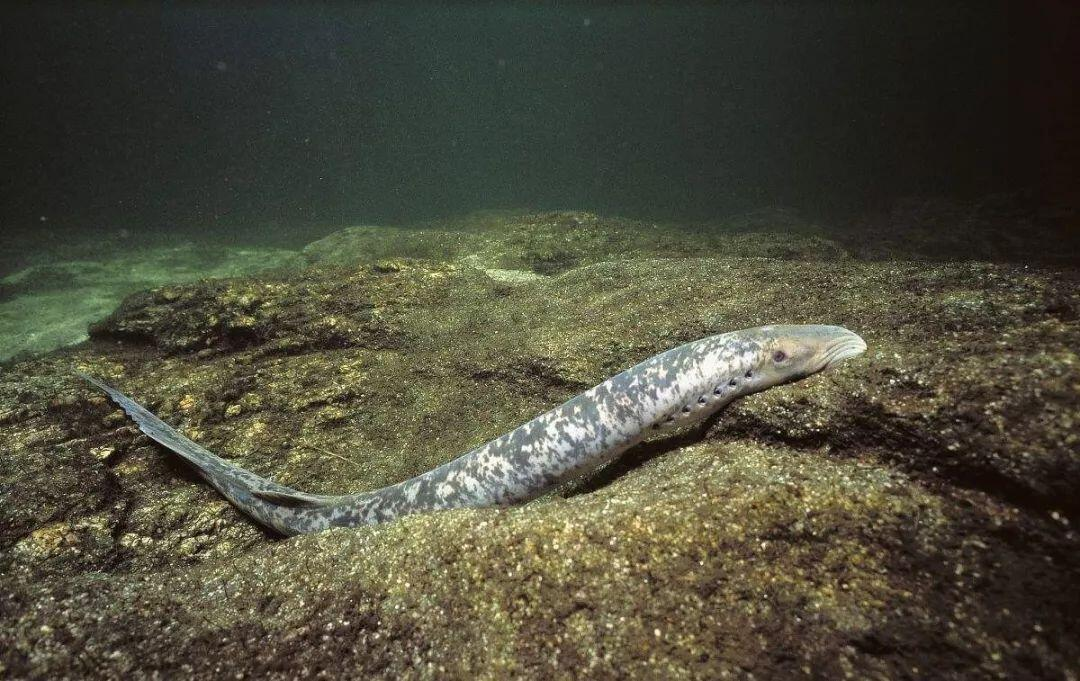
\includegraphics[width=8cm]{figures/lamprey_background.jpg}  % 引入图片源
\caption{Lamprey} \label{fig:Lamprey}  % 标题与标签
\end{figure}  % 图片结束
%%%%%%%% 图片 %%%%%%%%

\subsection{Restatement of the Problem }

\begin{itemize}  % 无序列表
\item An ecological simulation model that takes into account the interactions and impacts of species should be constructed to simulate and predict changes in the population of a species that can adaptively regulate sex ratios based on the availability of environmental resources.
\item Examine the relationship between the availability of natural resources and the sex ratio of the lamprey species. 
\item Analyse the implications for ecosystems of the ability of lamprey sex ratios to adapt to the availability of environmental resources. 
\item Analyse the implications for the lamprey species itself of the ability of sex ratios to adapt to the availability of environmental resources. 
\item Analyse the implications for species that parasitize lamprey bodies of the fact that lamprey sex ratios can adapt to the availability of environmental resources. 
\end{itemize}  % 无序列表结束

\subsection{Our Work}
In this paper, we establish Simulation Model with Environmental Sex.

Determination and Ecosystem Stability Assessment Model progressively and address four problems, which are listed below:
%%%%%%%% 图片 %%%%%%%%
\begin{figure}[H]  % 图片
\small
\centering  % 居中
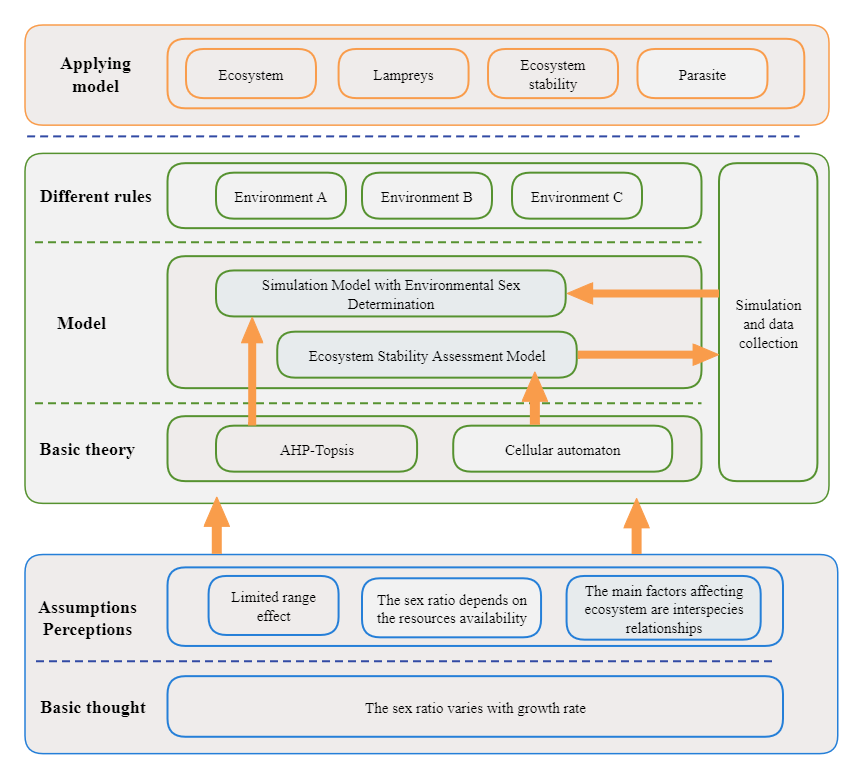
\includegraphics[width=15cm]{figures/architectural.png}  % 引入图片源
\caption{Our Work} \label{fig:Our Work}  % 标题与标签
\end{figure}  % 图片结束
%%%%%%%% 图片 %%%%%%%%

\section{Assumptions and Justifications}
To simplify the problem and make it convenient for us to simulate real-life conditions, we make the following basic assumptions, each of which is properly justified. 
\begin{itemize}  % 无序列表
\item \textbf{The sex ratio of lampreys is solely dependent on the difference between the surrounding food quantity and the surrounding lamprey quantity.} The gender ratio of lampreys depends on the growth rate of lampreys, and the growth rate is mainly determined by the abundance of food.\cite{1}

\item \textbf{The organisms within the ecosystem are only influenced by the limited-range environment in their surroundings.} It reflects the reality of how entities interact in nature, where the influence of one part on another is often limited by distance or connectivity. 

\item \textbf{The factors influencing ecosystem stability mainly come from the species population variability, the length of the cycle of change in the population, ecosystem resilience, and ecosystem resistance.} Since the constructed ecosystem only consists of predators and prey, only these four primary factors above need to be considered, and there is no need to account for other secondary factors, such as climate change or water quality fluctuations.

\item \textbf{The space in the ecosystem is assumed to be uniform and homogeneous. The effects of the space on the organisms within it are isotropic.} By treating space as uniform and homogeneous, models can capture essential patterns and behaviors of complex systems with fewer parameters, making simulation and analysis more tractable.

\item \textbf{Male and female lampreys have different resource requirements and predatory abilities, and the reproductive capacities of lampreys at different sex ratios are also different.}The gonadal structures of male and female lampreys are quite different, with females requiring more energy to grow. They therefore need to consume more food. Female lampreys in the same environment tend to be longer than males, and their different body result in different hunting abilities.\cite{2}

\item \textbf{When assessing the stability of an ecosystem, the decision criteria used to evaluate alternative solutions are mutually independent.} By maintaining the independence of criteria, the AHP-TOPSIS model accurately ranks alternative solutions based on a comprehensive score that accurately reflects their performance across all considered dimensions.


\end{itemize}  % 无序列表结束


\section{Notations}
%%%%%%%%%%%%%%%%%%%%%%%% 三线表 %%%%%%%%%%%%%%%%%%%%%%%%
\begin{table}[H]
    \centering
   
    \begin{tabular}{ccc}
    \hline
        \textbf{Symbol } & \textbf{Description } & \textbf{Unit } \\ \hline
        ${\displaystyle {\mathcal {L}}}$ & \thead{Lattice, used to represent the spatial layout of cells} & null \\ 
        ${\displaystyle {\mathcal {E}}}_A$ & \thead{Represent a finite set of states (species A)} & null \\ 
        ${\displaystyle {\mathcal {N}}}$ & \thead{Determines which neighboring cell states that\\
         will affect the update of the current cell state} & null \\ 
        ${\displaystyle {\mathcal {R}}}$ & \thead{Determines the next state of the cell\\ based on the current state of the cell and its neighbors} & null \\
        $N_{A}/N_{A}(\tau_{CA})$ & \thead{Represents the number of species A,\\ usually a function of $\tau_{CA}$} & year \\
        $\tau_{CA}$ & \thead{Represents the time variable in the CA model $\tau_{CA} \in \mathbb{Z}^{*}$} & null \\ 
        $State(i,j)_{lamp}$   & \thead{Represents the lamprey's state of the cell at i, j, which $\in {\displaystyle {\mathcal {E}}}_1$} & null \\ 
        $State(i,j)_{prey}$   & \thead{Represents the lamprey's prey's state\\ of the cell at i, j, which $\in {\displaystyle {\mathcal {E}}}_2$} & null \\ 
        \hline
    \end{tabular}
    \caption{\textbf{Notations}}
    \label{table}
\end{table}
%%%%%%%%%%%%%%%%%%%%%% 三线表结束 %%%%%%%%%%%%%%%%%%%%%%

%%%%%%%%%%%%%%%%%%%%%%%% 三线表 %%%%%%%%%%%%%%%%%%%%%%%%
\begin{table}[H]
    \centering
   
    \begin{tabular}{ccc}
    \hline
        $Rep_{capa}$ & \thead{Reflects the ability of a population to reproduce} & null \\
        $Res_{req}$ &  \thead{The group's demand for environmental resources} & null \\
        $Prey_{ab}$ &  \thead{The group's predatory ability} & null \\
        $Env_{A}$ &  \thead{Prey, Lampreys that can change gender\\ according to environmental adaptability} & null \\
        $Env_{B}$ & \thead{Prey, Lampreys that cannot alter its sex\\ (Lampreys are born with a 1:1 sex ratio)} & null \\
        $Env_{C}$ & \thead{Prey, Lampreys with a sex ratio of 1:1\\ (The sex ratio of surviving lampreys is always 1:1)}  & null \\
        \hline
    \end{tabular}
    \caption{\textbf{Continuation Table of Notations}}
    \label{table}
\end{table}
%%%%%%%%%%%%%%%%%%%%%% 三线表结束 %%%%%%%%%%%%%%%%%%%%%%

\section{Model 1: Simulation Model with Environmental Sex Determination}

Before proceeding, it is important to note that \textbf{we are discussing the adaptive change in sex ratio in response to the environmental resource availability}. 

From the perspective of mathematics, because the sex ratio of the lamprey population will change adaptively due to the availability of resources in the environment, this means that the dynamic equation representing the specific characteristics of the population adds a correction term about sex (hereinafter referred to as: \textbf{sex correction term}). At the same time, it is a biological fact that male and female lampreys have different predatory abilities, food quantity requirements, and reproductive contributions to the group. (These differences will be explained in more detail below.) Therefore, the addition of the sex correction term will have an impact on the solution of equation which representing the ecosystem and the lamprey population.  Therefore, during the subsequent simulation and evaluation process, we do not fit a large amount of specific data, to obtain parameters and rules that strictly adhere to reality. Starting from a general perspective, we will study an arbitrary parameter and rule, compare and observe the simulation results with and without the sex correction term, analyze and evaluate the significance of adding the sex correction term, and then examine the impact of the ability of sex ratios to adapt to the availability of environmental resources.

\subsection{Model Overview}

Our model is based on the concept of cellular automata. This is because, as observed in biology, it is often only the environment within a limited range that affects individuals within a species. Similarly, an individual can only affect a limited extent of its surroundings. This is consistent with the feature of cellular automata that the state transition of the cell is only related to the limited neighborhood. The model building process is shown in \textbf{Figure 3}. Therefore, to simulate species population dynamics and their food supply, it is only necessary to \textbf{expand the definition of cellular automata} and establish reasonable rules based on the impact of resource availability on sex ratios.

%%%%%%%% 图片 %%%%%%%%
\begin{figure}[h]  % 图片
\small
\centering  % 居中
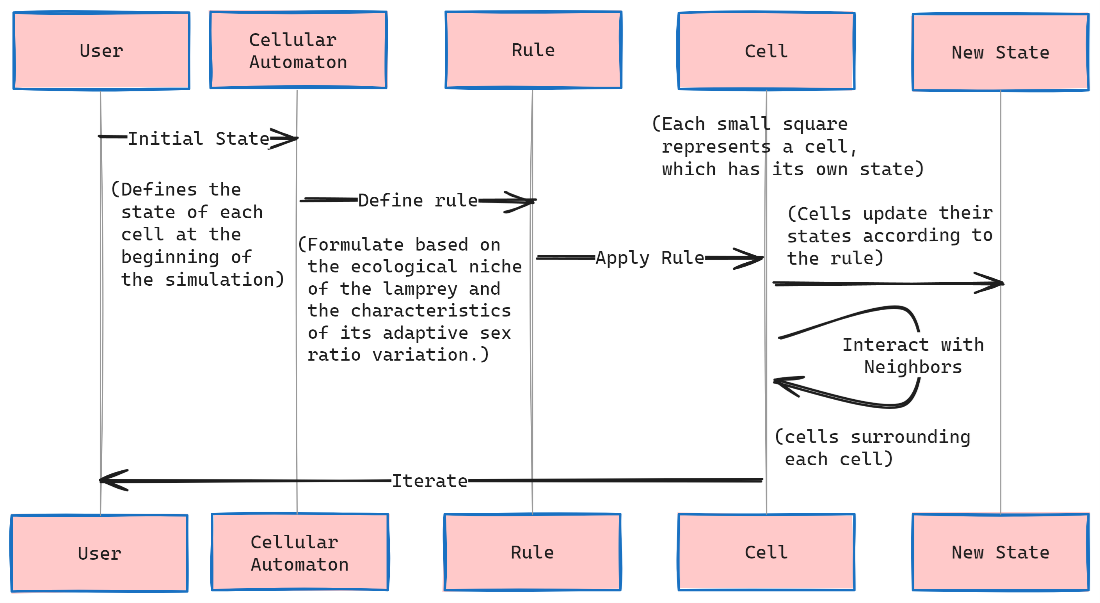
\includegraphics[width=12cm]{CA.png}  % 引入图片源
\caption{Model Design Process} \label{fig:Model Design Process}  % 标题与标签
\end{figure}  % 图片结束
%%%%%%%% 图片 %%%%%%%%

A Cellular Automata (CA) is a discrete computational model studied in automata theory. It generates a new generation based on a fixed rule (usually a mathematical function) \cite{3} that determines the new state of each cell based on the current state of the cell and the states of the cells in its neighborhood. The updating rule for the cells is typically the same for each cell and is applied to the entire grid simultaneously \cite{4}. 

As described above, a general cellular automaton is defined by a lattice ${\displaystyle {\mathcal {L}}}$, a state space ${\displaystyle {\mathcal {E}}}$, a neighborhood ${\displaystyle {\mathcal {N}}}$, and a rule ${\displaystyle {\mathcal {R}}}$ \cite{5}. But our model extends the definition based on cellular automata. Our model uses two sets of states to represent two different organisms, allowing us to simulate changes in the ecosystem of non-single ecological species. So, we stipulate that for a unit grid, two state information can be stored: one( ${\displaystyle {\mathcal {E}}}_1$ ) for the first creature and one( ${\displaystyle {\mathcal {E}}}_2$ ) for the second creature. The formal definition is a quintuple containing five sets:

\begin{align}
CA_{modified} \overset{def}{=} ({\displaystyle {\mathcal {L}}}, {\displaystyle {\mathcal {E}}}_1, {\displaystyle {\mathcal {E}}}_2, {\displaystyle {\mathcal {N}}}, {\displaystyle {\mathcal {R}}})
\end{align}

Specifically, ${\displaystyle {\mathcal {L}}}$ is a 2-dimensional grid used to represent the spatial layout of cells. ${\displaystyle {\mathcal {E}}}_1$ and ${\displaystyle {\mathcal {E}}}_2$  represent a finite set of states, and each cell is in a certain state in ${\displaystyle {\mathcal {E}}}_1 \times {\displaystyle {\mathcal {E}}}_2 $ at any time. ${\displaystyle {\mathcal {N}}}$ is the neighborhood definition, which determines which neighboring cell states will affect the update of the current cell state. And ${\displaystyle {\mathcal {R}}}: ({\displaystyle {\mathcal {E}}}_1 \times {\displaystyle {\mathcal {E}}}_2 )^{\left|{\displaystyle {\mathcal {N}}}\right|} \rightarrow {\displaystyle {\mathcal {E}}}_1 \times {\displaystyle {\mathcal {E}}}_2 $ is the conversion function, which determines the next state of the cell based on the current state of the cell and its neighbors. Here $\left|{\displaystyle {\mathcal {N}}}\right|$ is the number of cells in neighborhood ${\displaystyle {\mathcal {N}}}$.


\subsection{Creation and Assumptions of the Simulation Program}

According to the relevant literature \cite{6}, we have learned that without the interference of human factors, such as human predating and killing, sea lampreys basically have no natural enemies. Therefore, our first step is to construct a model that only considers the interaction between the sea lamprey and the prey that the sea lamprey hunts.

Since the size of the living environment is almost infinite compared to an individual lamprey, we can assume that the lattice ${\displaystyle {\mathcal {L}}}$ used for the simulation has no boundaries. However, when actually performing the simulation operations, due to the limitations of the computer, infinite boundaries cannot be considered. Therefore, we treat the top row as adjacent to the bottom row, and the left column as adjacent to the right column.

When simulating the model, each sea lamprey is assumed to have three states, namely absence (0), male survival (1) and female survival (2). That is ${\displaystyle {\mathcal {E}}}_1 = \{0, 1, 2\}$ to mean state of lamprey. And each prey is assumed to have two states, namely absence (0), alive (1). That is ${\displaystyle {\mathcal {E}}}_2 = \{0, 1\}$to mean state of prey.

Although the actual situation is that the sex of a sea lamprey is not obvious in the larval stage, it will \textbf{become female or male with different probabilities in near adulthood due to different resource availability} \cite{7}. However, considering that resource consumption during the larval stage is almost negligible, and to facilitate the simulation, when writing the rules ${\displaystyle {\mathcal {R}}}$, we assume that sea lampreys will have different birth probabilities of sex according to the current environmental resource availability. At the same time, considering that adult sea lampreys still have a probability of sex reversal in practice, we have included a little transition probability related to the current environmental resource availability in the rules ${\displaystyle {\mathcal {R}}}$. We also propose that for lampreys, \textbf{environmental resources are related to the abundance of nearby prey}.

Finally, before the simulation, we set the number of surviving prey, surviving female lampreys and surviving male lampreys at the initial time ($\tau_{CA} = 0$) and randomly assigned them to the environment by the program.

\subsection{Qualitative Description of Ecological Laws and Definition of Rule ${\displaystyle {\mathcal {R}}}$}

\subsubsection{About Lamprey}
Consider group density first. Considering interspecific competition, there cannot be too many lampreys in a given space, otherwise death will occur due to excessive density and overcrowding of the population. This is reflected in the rule ${\displaystyle {\mathcal {R}}}$, i.e. the number of lampreys in the neighbourhood ${\displaystyle {\mathcal {N}}}$ of a cell cannot exceed a constant, otherwise the cell's state $State(i,j)_{lamp}$ will die in the next moment, or it cannot go from $State(i,j)_{lamp}= 0$ to $State(i,j)_{lamp}= 1\,or\,2$, i.e. reproduction occurs.

Secondly, consider the reproductive capacity. In actual research, it was found that female lamprey contributes much more to the reproductive capacity of the lamprey population than male lamprey \cite{2}. Therefore, we define \textbf{Reproductive Capacity}:
\begin{align}
Rep_{capa} = N_f \times rep_f + N_m \times rep_m
\end{align}
 Where $N_f$ is the number of female lamprey, $N_m$ is the number of male lamprey, $rep_f$ is reproductive contribution coefficient of female, and $rep_m$ is reproductive contribution coefficient of male. Reflected in the rule ${\displaystyle {\mathcal {R}}}$, a cell which $State(i,j)_{lamp} = 0$ has the possibility of reproduction only when its reproductive capacity $Rep_{capa}$ in its neighborhood should be greater than a constant.

 Next, consider the group's demand for environmental resources. Here we have assumed that the demand for environmental resources is equivalent to the demand for food. In order to continue to survive or reproduce, the amount of food, i.e. the number of prey in the simulation, must be greater than the group's demand for food. Experiments and theory have shown that, compared to males, female lampreys have a greater need for things \cite{2}. Therefore, we define \textbf{Resource requirements}:

\begin{align}
Res_{req} = N_f \times res_f + N_m \times res_m
\end{align}
 Where $N_f$ is the number of female lamprey, $N_m$ is the number of male lamprey, $res_f$ is environmental demand factor of female, and $res_m$ is environmental demand factor of male. Reflected in the rule ${\displaystyle {\mathcal {R}}}$, a cell which $State(i,j)_{lamp} = 0$ has the possibility of reproduction only when its reproductive capacity $Res_{req}$ in its neighborhood should be less than the amount of food (that is, the amount of lamprey's prey).

\subsubsection{About Lamprey's prey}

For lamprey prey (hereafter referred to as prey), the first thing to consider is population density. Because of interspecific competition, there cannot be too many prey in the same space, otherwise they will die due to excessive population density and overcrowding. This is reflected in the rule ${\displaystyle {\mathcal {R}}}$, that the number of prey in a cell's neighbourhood ${\displaystyle {\mathcal {N}}}$ cannot exceed a constant, otherwise the cell's state $State(i,j)_{prey}$ will die in the next moment, or it cannot go from $State(i,j)_{prey}= 0$ to $State(i,j)_{prey}= 1$, i.e. reproduction occurs.

If we then consider the relationship between predator and prey, in order to continue to survive or reproduce, there cannot be too many predators in the environment. For lampreys, their predator is the lamprey, so there cannot be too many predators in the environment. In other words, there cannot be too many lampreys in the environment. According to experimental data, it is shown that the predatory ability of male lampreys is stronger than that of female lampreys, so we define the \textbf{Predatory Ability}:
\begin{align}
Prey_{ab} = N_f \times pre_f + N_m \times pre_m
\end{align}
Where $N_f$ is the number of female lamprey, $N_m$ is the number of male lamprey, $pre_f$ is predatory factor of female, and $pre_m$ is predatory factor of male. This is reflected in the rule ${\displaystyle {\mathcal {R}}}$ of the model, i.e. lamprey’s predatory ability $Prey_{ab}$ cannot be greater than a constant, otherwise the prey cannot reproduce or continue to survive.

\subsubsection{Rule Modifications for Breeding Offspring}
Now comes the most exciting part. As we said before, the lamprey has the ability to adapt its sex to the environment. Therefore, combined with the related assumptions mentioned above, we set the reproductive part of the lamprey in the rule ${\displaystyle {\mathcal {R}}}$, this means that if a cell which $State(i,j)_{lamp}= 0$ meets all the conditions for reproduction which we discussed above, its $State(i,j)_{lamp}$ will become $1$ (male) and $2$ (female). Whether it becomes $1$ (male) or $2$ (female) depends on the abundance of food in the environment. We believe that the probability of becoming $2$ (female) is a linear function of the food abundance, and the \textbf{Food Abundance} is defined as $Food_{abun} = N_{prey} - Res_{req}$ , where $N_{prey}$ is the number of lamprey's prey in the neighbourhood. And the linear function is:
\begin{align}
P_{female} = k\times Food_{abun} + b
\end{align}
Where $P_{female}$ is the \textbf{probability of giving birth to a female}, and $k$, $b$ are the two coefficients of the linear equation. The equation shows that the more abundant the food, the higher the proportion of females. This corresponds to the actual laws of nature and is therefore a reasonable equation.

\subsection{Simulation Process and Results}
We will now try to run a simulation program using the model we have created above. Before the simulation we have the following settings:

$\tau_{CA} = 0, N_f(0) = 450, N_m(0) = 450, N_{prey}(0) = 2400. \text{And } \tau_{CA} \in \left[0, 100\right]$, this means we will do 100 iterations.
$\left|{\displaystyle {\mathcal {N}}} \right| = 9$, This means that for a cell, its neighbor ${\displaystyle {\mathcal {N}}}$ is a $3\times 3$ area centered on itself. And ${\displaystyle {\mathcal {L}}}$ is a $100\times 100$ grid. And  we treat the top row as adjacent to the bottom row, and the left column as adjacent to the right column as we said above. Finally, We have already discussed ${\displaystyle {\mathcal {S}}}$ and ${\displaystyle {\mathcal {R}}}$ in 4.2 and 4.3. They are set here according to the results of the discussion.


The following \textbf{Figure 4} is the result of the simulation program. In each sub-figure, the left image is a visualisation of the number and distribution of lampreys. Purple indicates that there are no lampreys here, green indicates that there are male lampreys here and yellow indicates that there are female lampreys here. The image on the right is a visualisation of the number and distribution of prey. Black indicates that there is no prey here and yellow indicates that there is prey here.

\begin{figure}[H]
  \centering
  % 第一行
  \begin{subfigure}[b]{0.45\textwidth}
    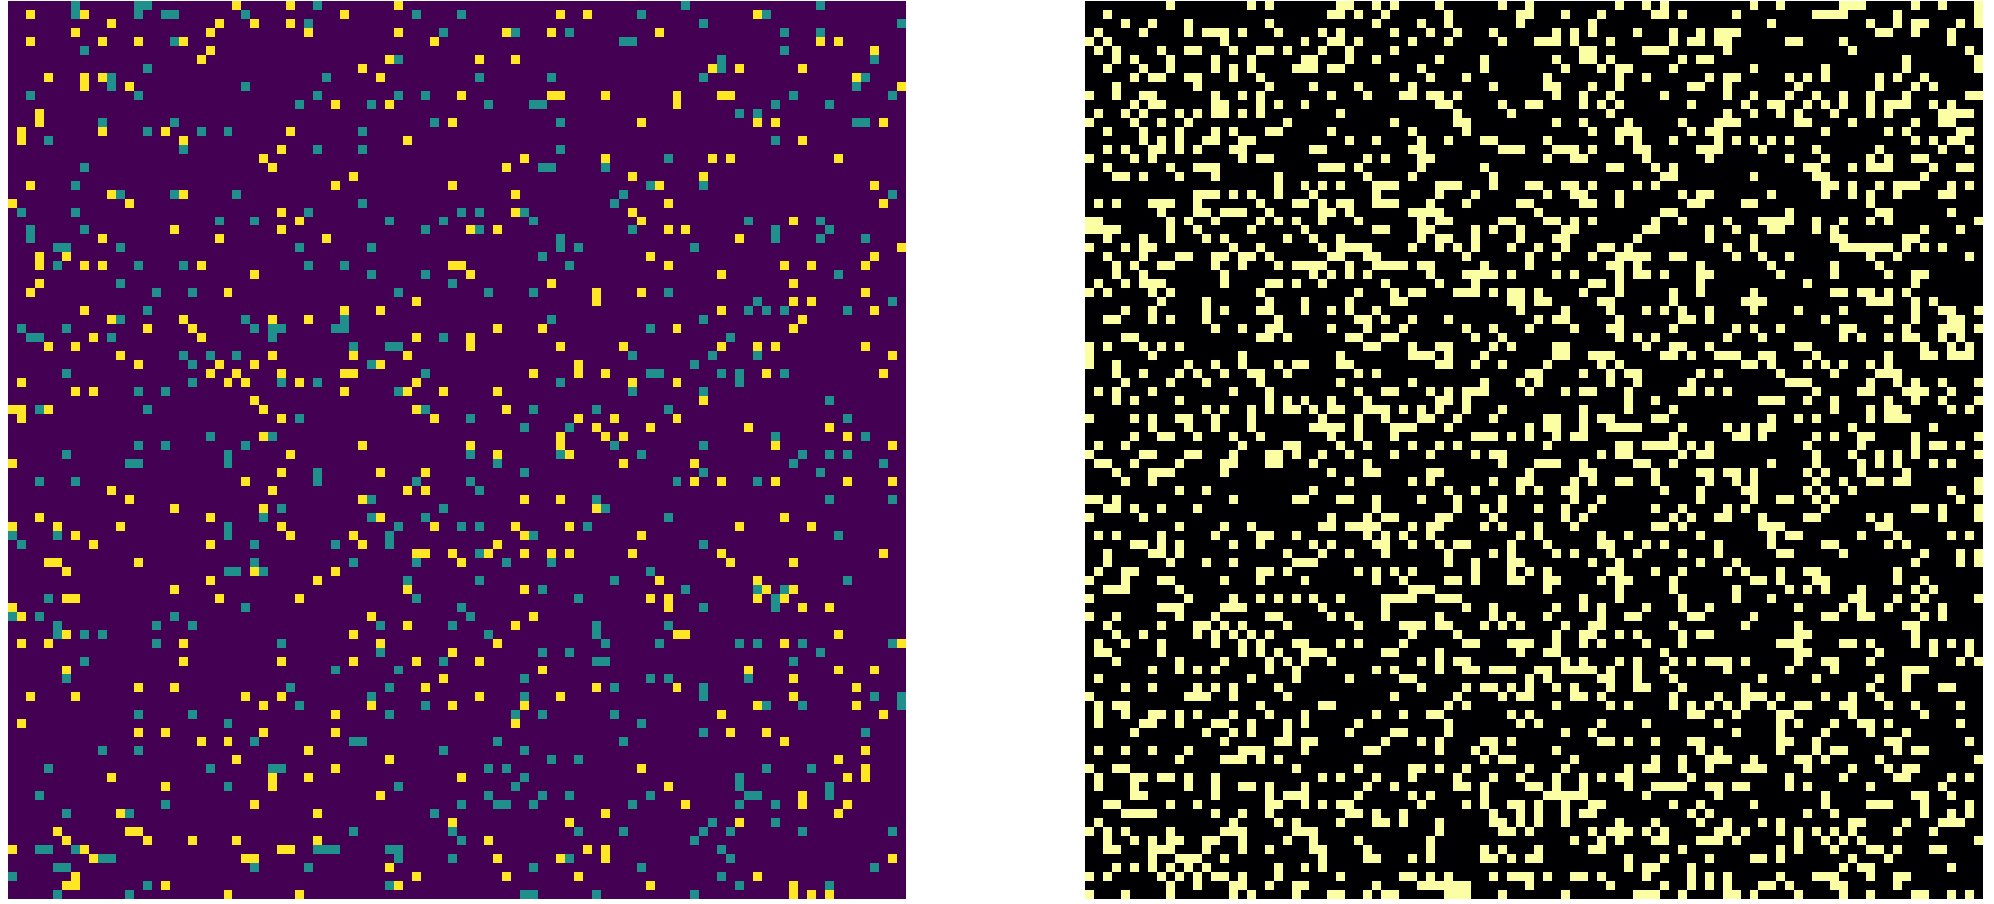
\includegraphics[width=\textwidth]{figures/NormalSimulation_1.png}
    \caption{$\tau_{CA} = 0$}
    \label{fig:sub1}
  \end{subfigure}
  \hfill
  \begin{subfigure}[b]{0.45\textwidth}
    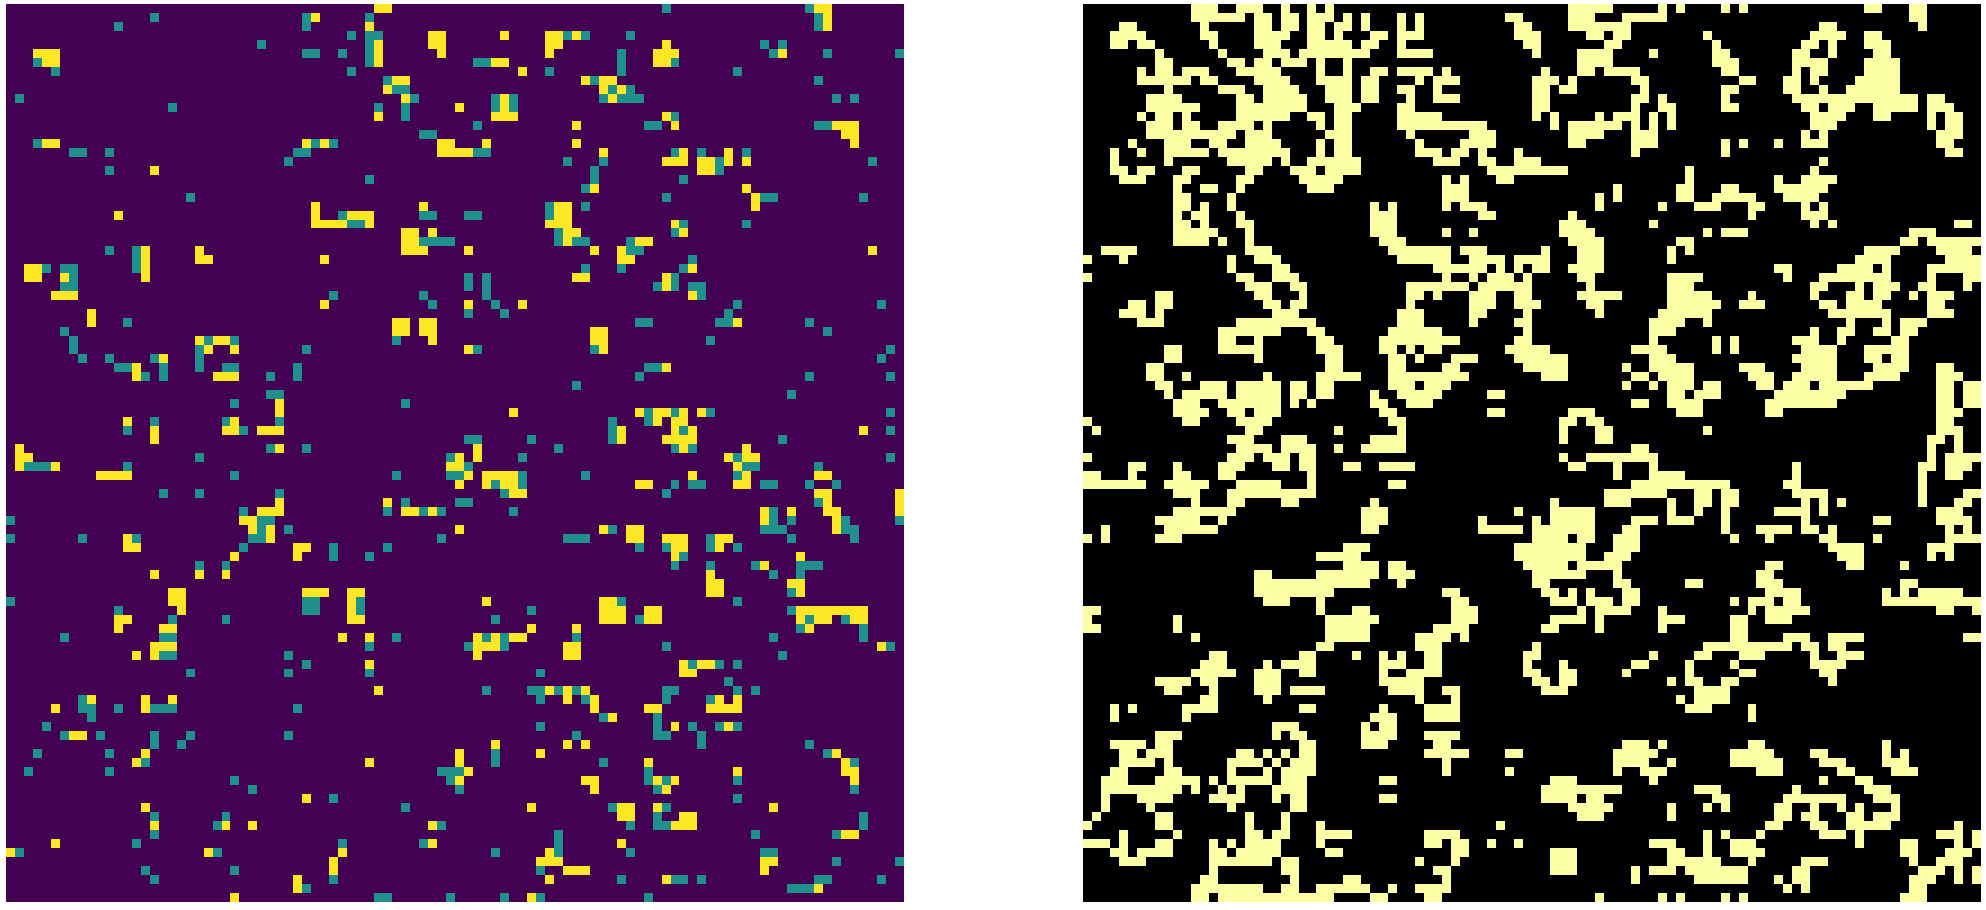
\includegraphics[width=\textwidth]{figures/NormalSimulation_2.png}
    \caption{$\tau_{CA} = 20$}
    \label{fig:sub2}
  \end{subfigure}

  % 水平分隔线
  \vspace*{5pt} % 在分隔线前后添加一些垂直空间
  \hrule % 默认页面宽度的水平线
  \vspace*{5pt} % 调整空间以适配布局
  
  % 第二行
  \begin{subfigure}[b]{0.45\textwidth}
    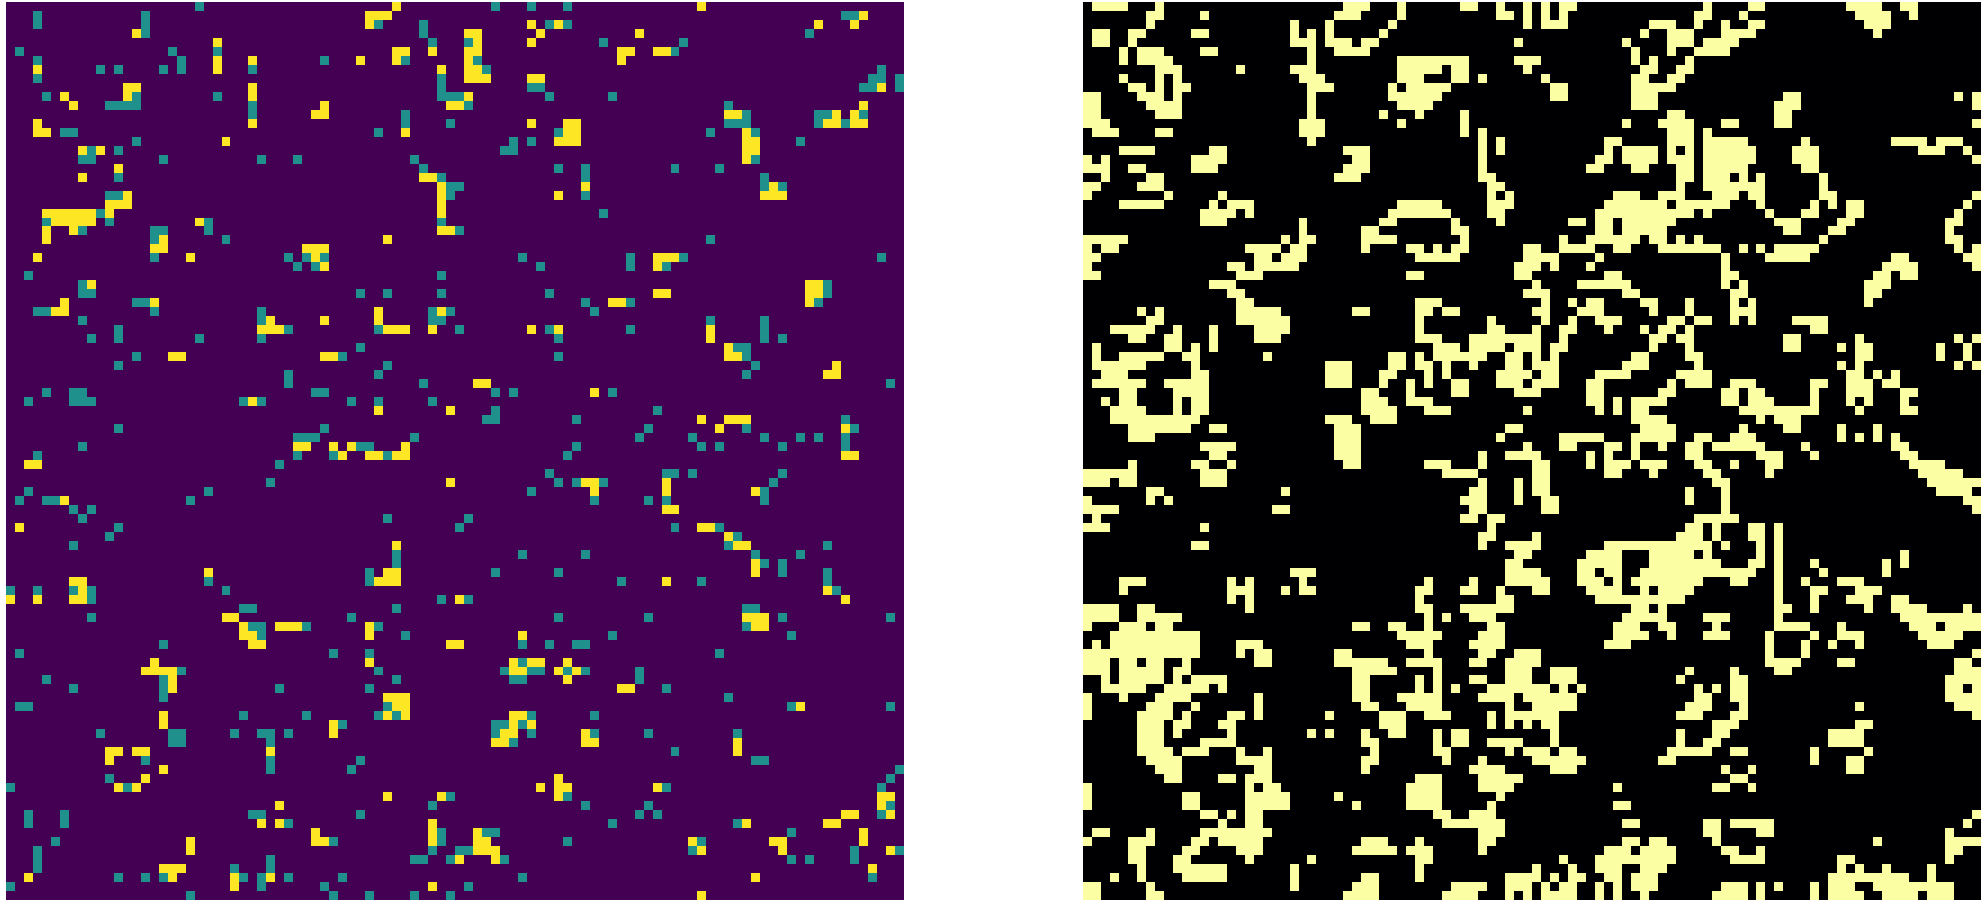
\includegraphics[width=\textwidth]{figures/NormalSimulation_3.png}
    \caption{$\tau_{CA} = 40$}
    \label{fig:sub3}
  \end{subfigure}
  \hfill
  \begin{subfigure}[b]{0.45\textwidth}
    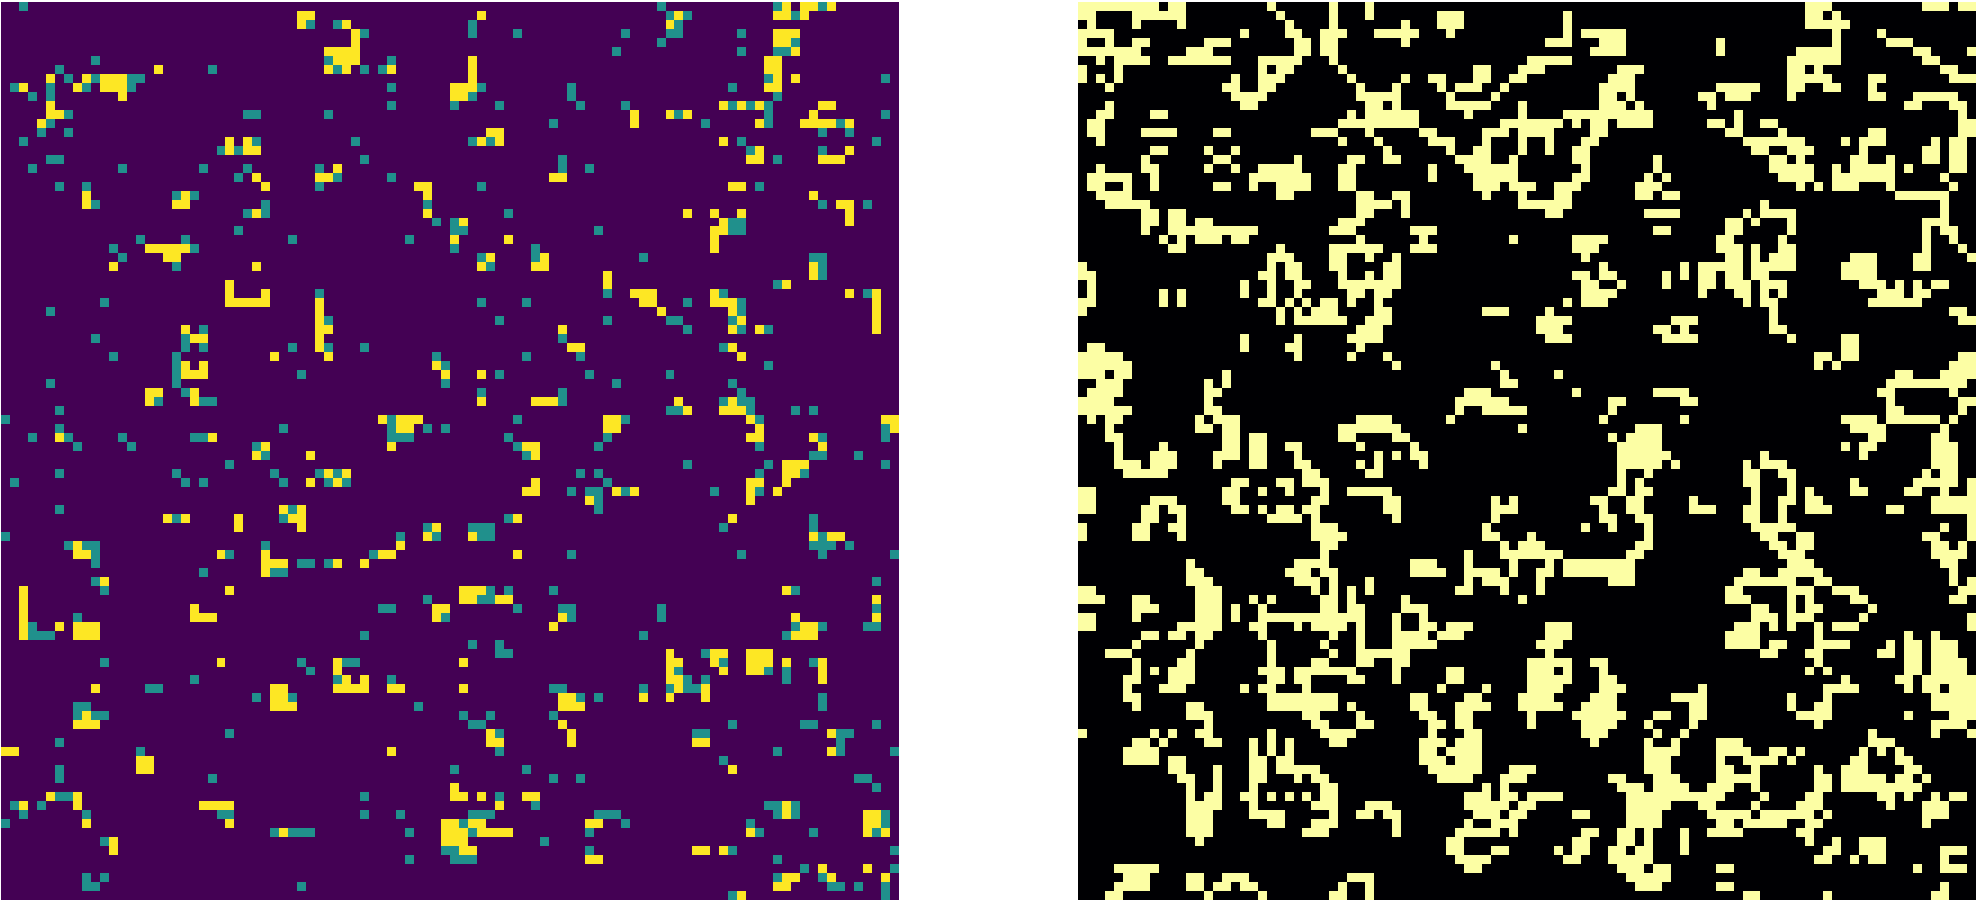
\includegraphics[width=\textwidth]{figures/NormalSimulation_4.png}
    \caption{$\tau_{CA} = 60$}
    \label{fig:sub4}
  \end{subfigure}

  % 水平分隔线
  \vspace*{5pt} % 在分隔线前后添加一些垂直空间
  \hrule % 默认页面宽度的水平线
  \vspace*{5pt} % 调整空间以适配布局
  
  % 第三行
  \begin{subfigure}[b]{0.45\textwidth}
    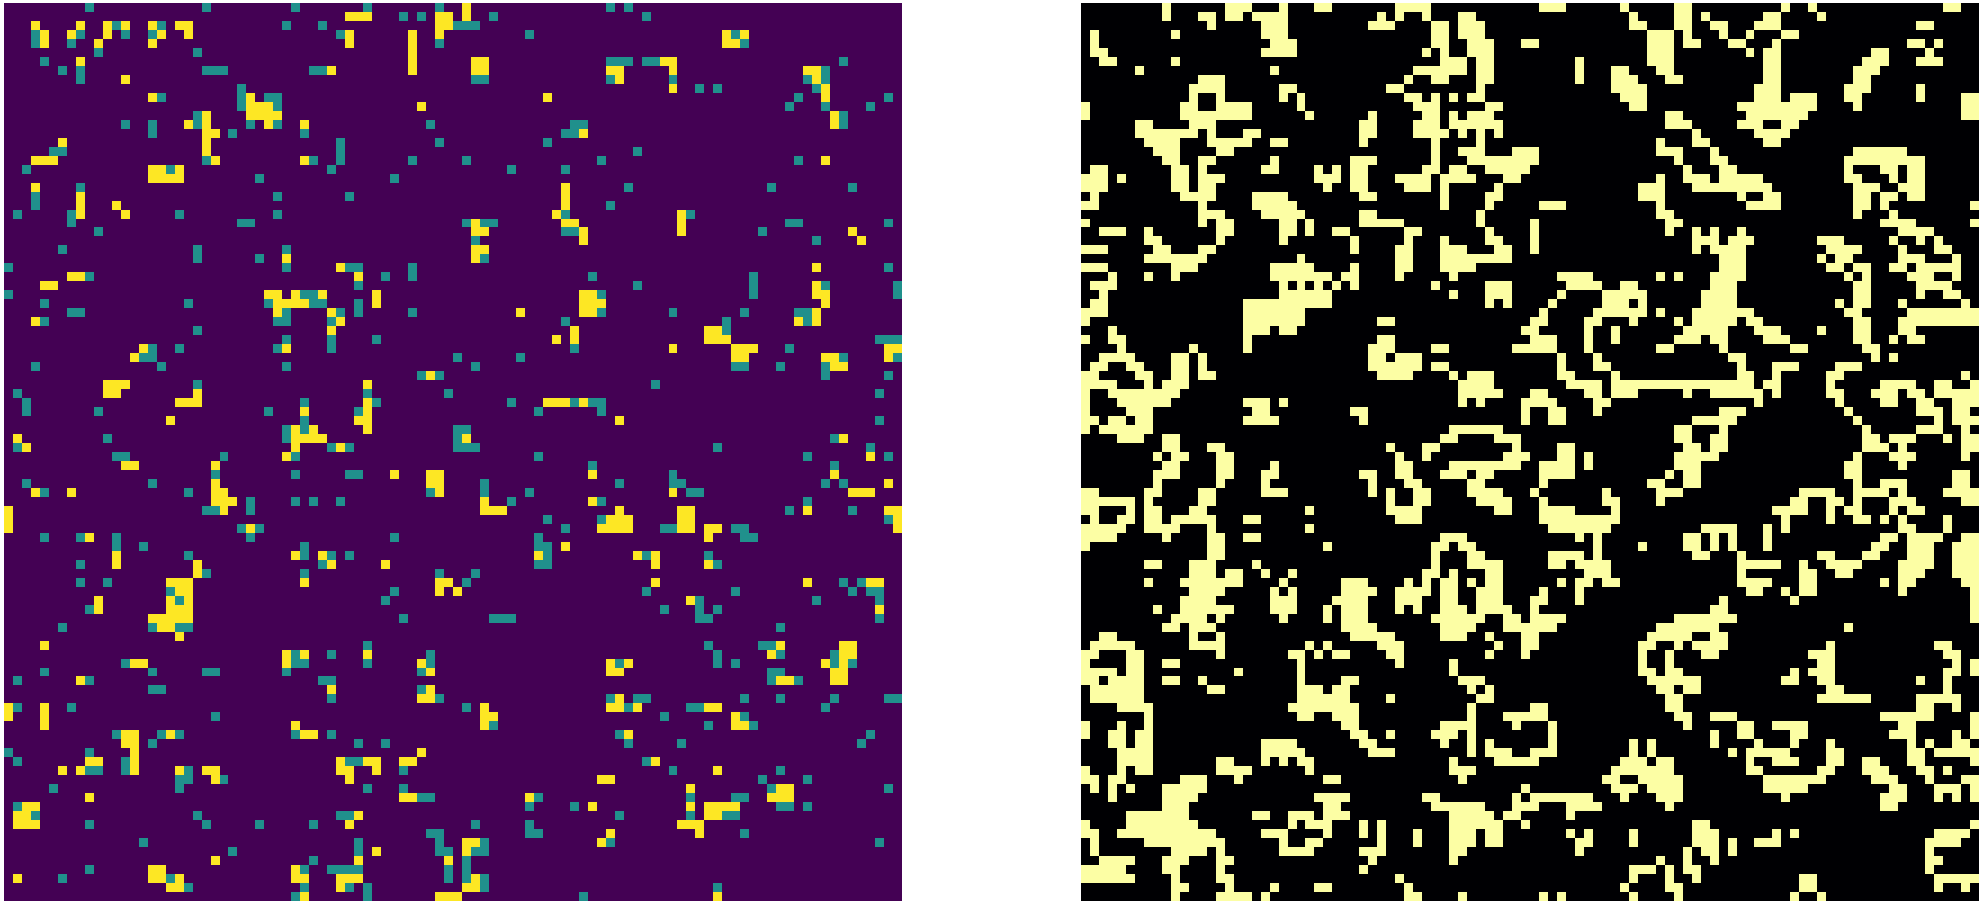
\includegraphics[width=\textwidth]{figures/NormalSimulation_5.png}
    \caption{$\tau_{CA} = 80$}
    \label{fig:sub5}
  \end{subfigure}
  \hfill
  \begin{subfigure}[b]{0.45\textwidth}
    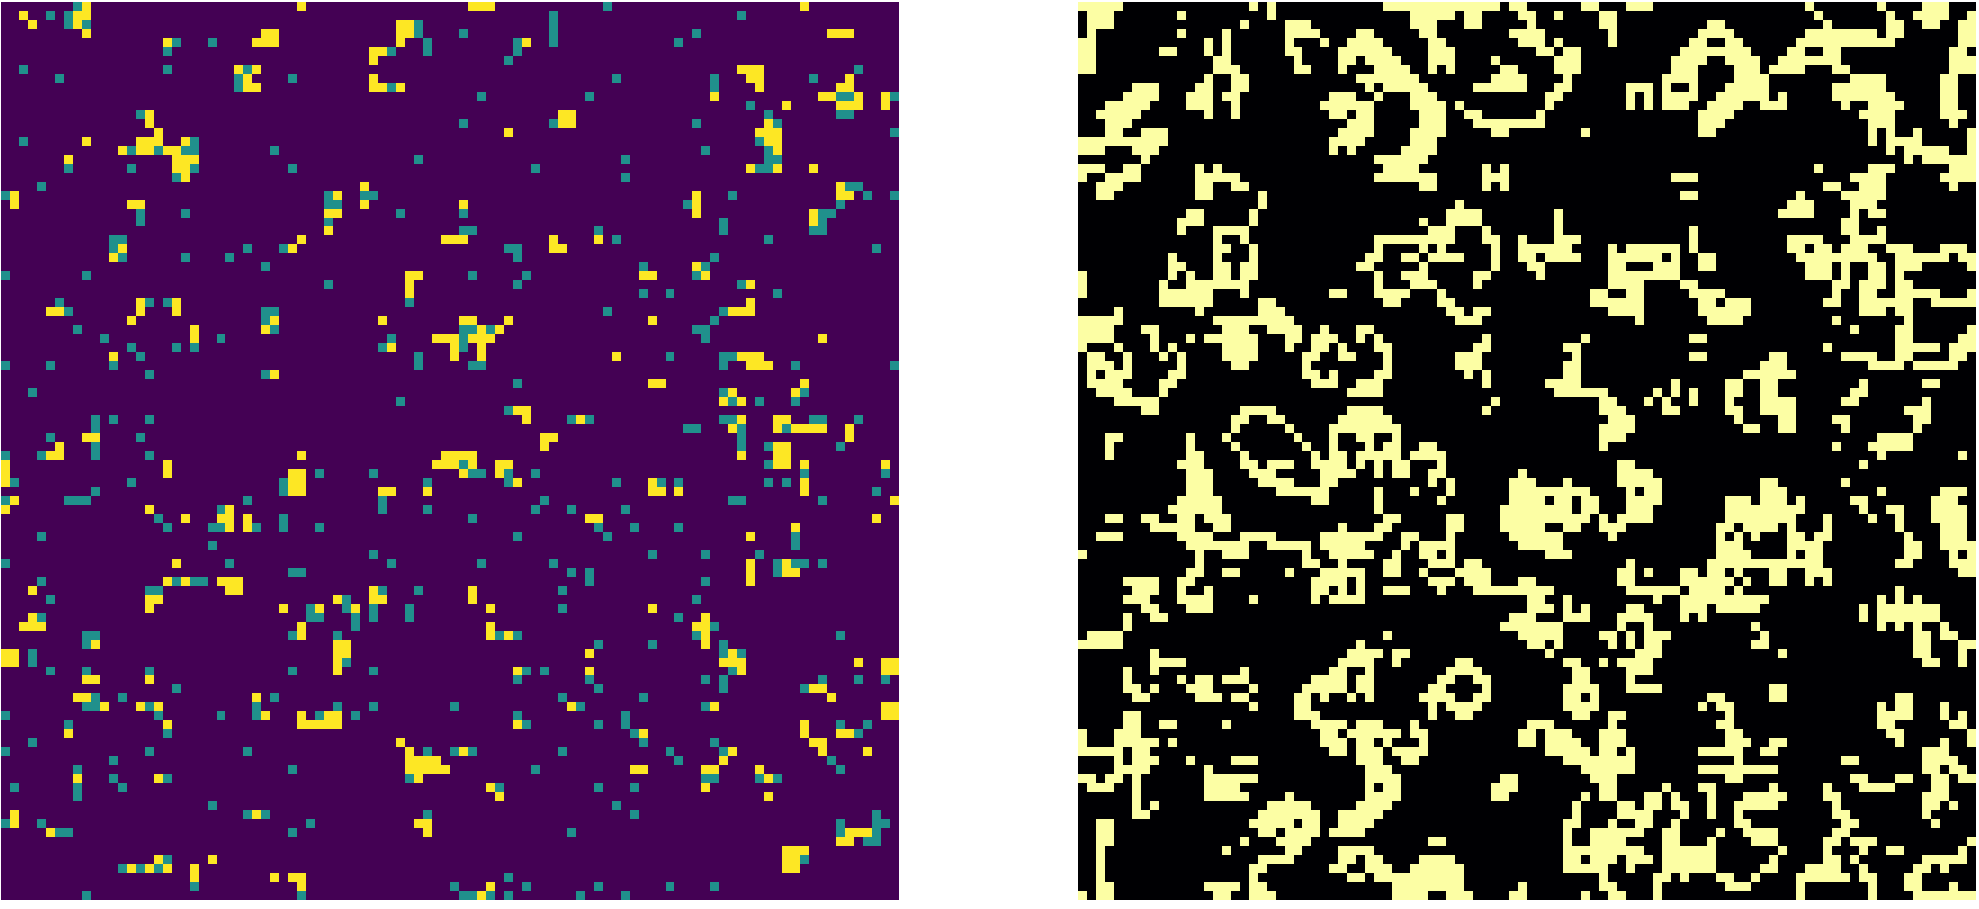
\includegraphics[width=\textwidth]{figures/NormalSimulation_6.png}
    \caption{$\tau_{CA} = 100$}
    \label{fig:sub6}
  \end{subfigure}
  
  \caption{Result of Simulation}
  \label{fig:Result of Simulation}
\end{figure}

% Finally, we also plotted the changing trend curves of the numbers of different species over time (see Figure 4).
% %%%%%%%% 图片 %%%%%%%%
% \begin{figure}[h]  % 图片
% \small
% \centering  % 居中
% 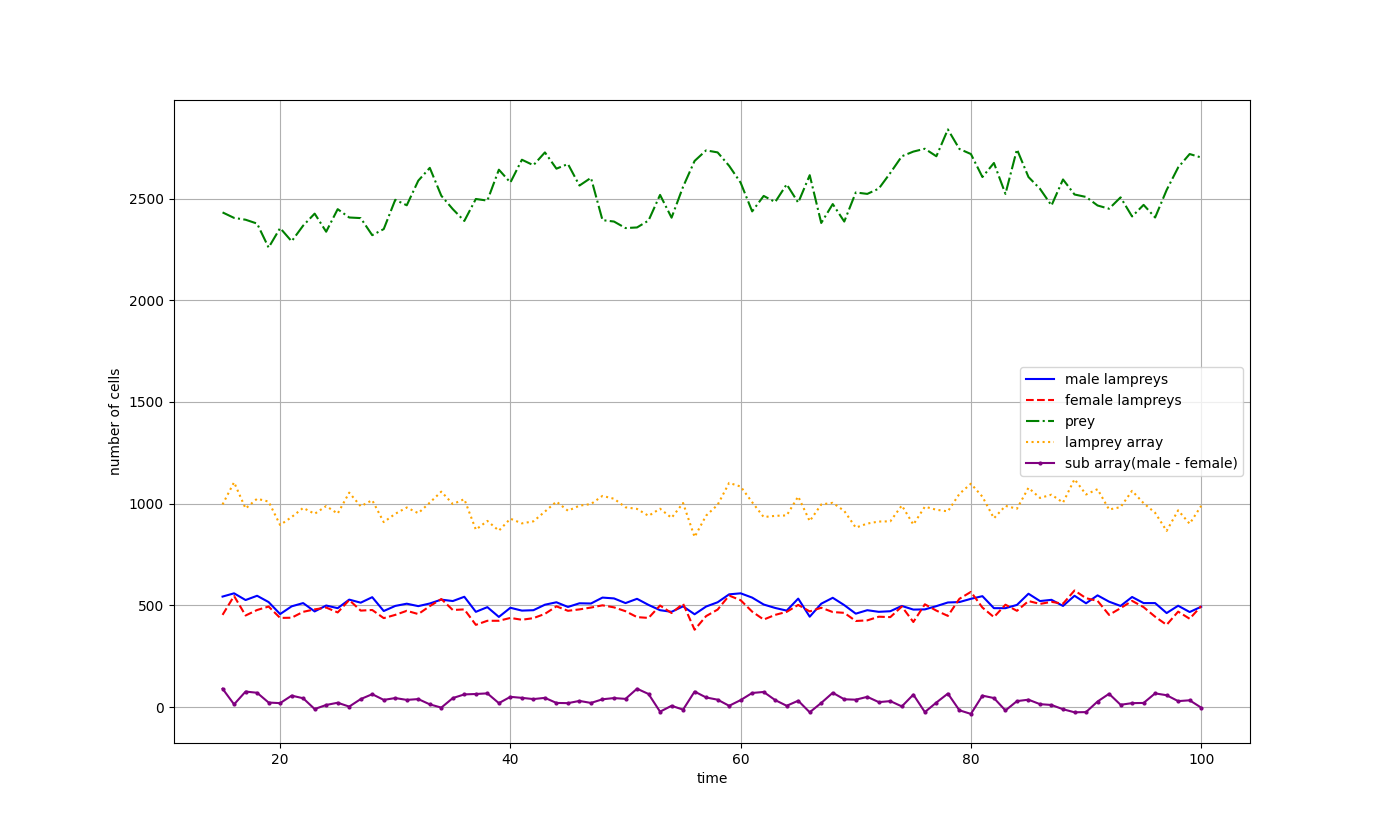
\includegraphics[width=\textwidth]{NormalSimulationResult.png}  % 引入图片源
% \caption{Species Number Change Curve} \label{fig:Species Number Change Curve}  % 标题与标签
% \end{figure}  % 图片结束
% %%%%%%%% 图片 %%%%%%%%

\section{Model 2: Ecological Stability Assessment Model}
\subsection{Model Overview}
To assess the stability of ecosystems under different scenarios, we quantify the stability of ecosystems. We assign a score to the stability of an ecosystem. After searching the relevant literature and combining the data we simulated in \textbf{Model 1}, we identified four factors that determine the stability of an ecosystem: the volatility of the number of species, the length of the cycle, the ecosystem's resistance and the ecosystem's resilience. 

Using the Analytic Hierarchy Process (AHP), we can derive the weights of the above four factors. 

Using Topsis, combined with the weights obtained using AHP, we can derive a score for ecosystem stability. 

\subsection{Determine the Weight}
\subsubsection{Build a Hierarchical Model}

%%%%%%%% 图片 %%%%%%%%
\begin{figure}[h]  % 图片
\small
\centering  % 居中
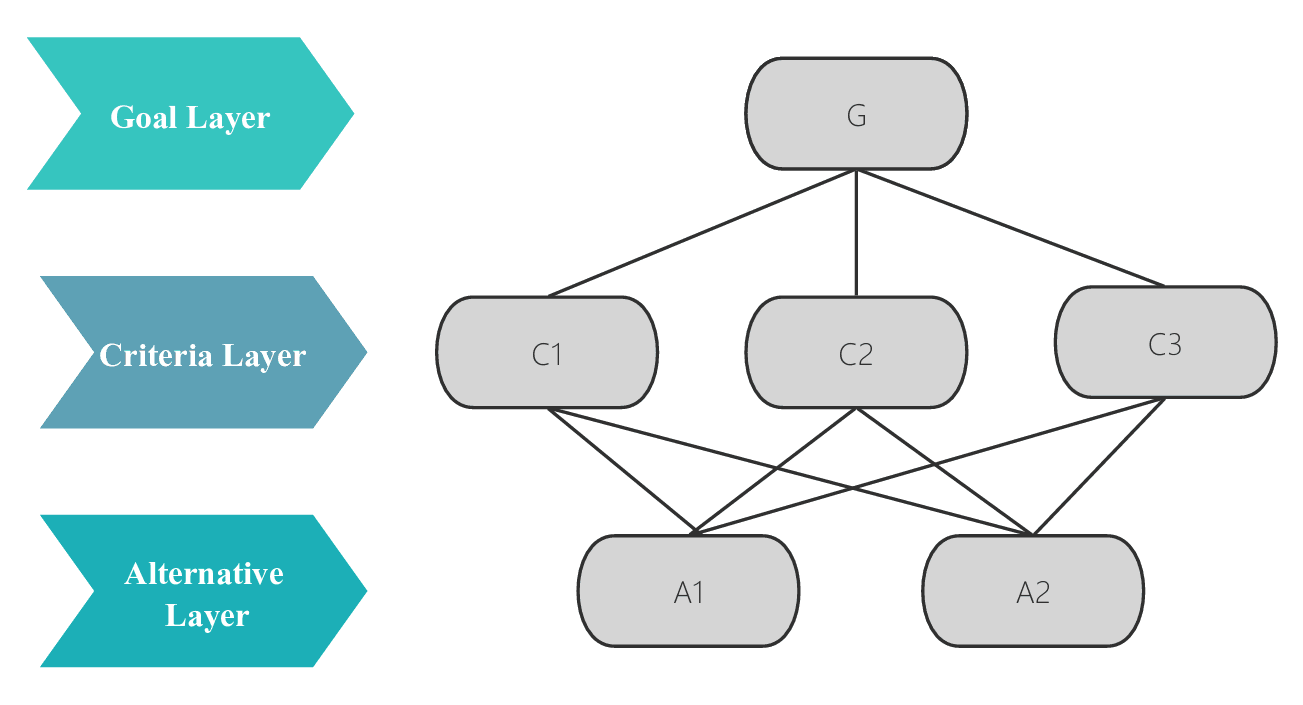
\includegraphics[width=0.75\textwidth]{Hierarchical_Model.png}  % 引入图片源
\caption{Hierarchical Model} \label{fig:Hierarchical Model}  % 标题与标签
\end{figure}  % 图片结束
%%%%%%%% 图片 %%%%%%%%

\textbf{Objective layer:} To assess the stability of the ecosystem. 

\textbf{Criteria Layer:}
\begin{itemize}
    \item Species Population Variability: Refers to the fluctuations in the numbers of species within the ecosystem. 
    \item The length of the cycle of change in the population: The duration of natural cycles within the ecosystem.
    \item Ecosystem Resilience: The ability of the ecosystem to recover from disturbances and return to its pre-disturbance state. 
    \item Ecosystem Resistance: The capacity of the ecosystem to withstand disturbances without significant changes in its structure and functions. 
\end{itemize}

\textbf{Alternative Layer:}

\begin{itemize}
    \item System $Env_{A}$: Prey and lampreys that can alter its sex. 

    \item System $Env_{B}$: Prey and lampreys that cannot alter its sex (Lampreys are born with a 1:1 sex ratio). 

    \item System $Env_{C}$: Prey and lampreys with a sex ratio of 1:1 (The sex ratio of surviving lampreys is always 1:1. Even if they are born with a sex ratio of 1:1, the sex ratio will differ after they have survived for some time due to the difference in feeding ability and energy requirements for growth between male and female lampreys). 
\end{itemize}

\subsubsection{Constructing Pairwise Comparison Matrix}
The weights were calculated using the two-by-two comparison method of assigning values to the indicators, and a pairwise comparison matrix (A) was constructed, where the meaning of the matrix element $a_{ij}$ is the importance of the indicator i relative to the indicator j. 

\subsubsection{Consistency Check}
Calculate the maximum eigenvalue ($\lambda_{max}$) of the judgement matrix A. Then calculate the consistency indicators ($CI$), n is the order of the judgement matrix: $ CI=\frac{\lambda_{max}-n}{n-1} $

Then calculate the consistency ratio ($CR$): $ CR=\frac{CI}{RI} $

The $RI$ of the $4 \times 4$ matrix is 0.90. The consistency of the judgement matrix is considered acceptable if $CR$ is less than 0.1.

\subsubsection{Weight Criteria Calculation}
Normalize the pairwise comparison matrix (A), then sum the normalized matrix by rows and divide by n. Finally, obtain the weight vector ($w$) using the arithmetic mean method.
\begin{align}
w=(w_1,w_2,\ldots,w_n)\,\,\,, \quad\quad w_i=\frac{({\prod_{j=1}^{n}a_{ij})}^\frac{1}{n}}{\sum_{k=1}^{n}{({\prod_{j=1}^{n}a_{kj})}^\frac{1}{n}}},\left(i=1,2,\ldots,n\right)
\end{align}

\subsection{Calculating the Ecosystem Stability Score}
\subsubsection{Processing of Raw Data}
According to \textbf{Model 1}, the ecosystem $Env_{A}$, $Env_{B}$, and $Env_{C}$ are simulated. It is assumed that prior to time $\tau_{CA}={\tau_{CA}}_0$, the system exists in a state of stability, with the population of lampreys and the quantity of prey undergoing cyclic variations. At $\tau_{CA}={\tau_{CA}}_0$, a catastrophe occurs, resulting in a sudden decline in the prey, which subsequently returns to a state of stability after a duration of $m$ years.

Let's define the respective terms:
\begin{itemize}
    \item $T$ (in years): The duration of the lamprey population's periodic oscillations.
    \item $m$: The time it takes for an ecosystem to return to a stable state after a disaster.
    \item $U$: The average amplitude of the lamprey population as a function of time.
    \item $N_V$: The amount of prey available; $N_Z$: The quantity of lampreys following the restoration of stability subsequent to the catastrophe; $N_W$: The amount of prey available following the restoration of stability subsequent to the catastrophe.
    \item $\bar{N}_X$: The average population of lampreys; $\bar{N}_Y$: The average quantity of prey.
\end{itemize}

The following are the quantitatively defined four key factors that influence the stability of an ecosystem:	

Species Population Variability (a): $ a=\frac{U}{\bar{N}_X}+\frac{N_V}{\bar{N}_Y} $

The length of the cycle of change in the population (b): $b=T$

Ecosystem Resilience (c):  $c=m$

Ecosystem Resistance (d): $d=|\frac{\bar{N}_X-N_Z}{\bar{N}_X}|+|\frac{\bar{N}_Y-N_W}{\bar{N}_Y}|$

The original matrix $M_1$ can be obtained using the four equations provided. In this matrix, the elements ${m_{ij}}^\prime(i=1,2,\ldots,m,j=1,2,\ldots,n)$ represent the scores of the $j$-th factor for the $i$-th system. Here, $i=1, 2, 3$ correspond to systems $Env_{A}$, $Env_{B}$, $Env_{C}$ respectively, and $j=1, 2, 3, 4$ correspond to factors a, b, c, d respectively.

Factor b is a maximisation criterion and factors a, c and d are minimisation criteria. We directionalise the matrix $M_1$ to obtain the matrix $M_2$, then normalise $M_2$ to obtain the matrix $M_3$. Finally, we add the weights obtained from the equation to obtain the final normalised matrix $M$. We skip the intermediate steps and provide the final matrix $M$ directly:

\begin{align}
M=\left[\begin{matrix}m_{11}&\cdots&m_{1m}\\\vdots&\ddots&\vdots\\m_{n1}&\cdots&m_{nm}\\\end{matrix}\right]
\end{align}

\subsubsection{Calculating the Ecosystem Stability Score}

Define the maximum value ($M^+$) and the minimum value ($M^-$):
\begin{equation}
\begin{aligned}
M^+&=\left(M_1^+,M_2^+,\ldots,M_m^+\right)
\\
&=\left(\max{\left\{m_{11},m_{21},\ldots,m_{n1}\right\}},\max{\left\{m_{12},m_{22},\ldots,m_{n2}\right\},\ldots,\max{\left\{m_{1m},m_{2m},\ldots,m_{nm}\right\}}}\right)\\
M^-&=\left(M_1^-,M_2^-,\ldots,M_m^-\right)
\\
&=\left(\min{\left\{m_{11},m_{21},\ldots,m_{n1}\right\}},\min{\left\{m_{12},m_{22},\ldots,m_{n2}\right\},\ldots,\min{\left\{m_{1m},m_{2m},\ldots,m_{nm}\right\}}}\right)\\
\end{aligned}
\end{equation}




Define the distance of the $i$-th ($i = 1,2,\cdots, n$) evaluation object from the maximum value ($D_i^+$) and the minimum value ($D_i^-$)
\begin{align}
D_i^+=\sqrt{\sum_{j=1}^{m}\left(M_j^\pm m_{ij}\right)^2}\,\,\,, \quad\quad D_i^-=\sqrt{\sum_{j=1}^{m}\left(M_j^--m_{ij}\right)^2}
\end{align}

Therefore, the unnormalized score for the $i$-th ($i = 1,2,\cdots, n$) evaluation object ($S_i$) can be calculated, and finally, normalize the scores and convert them to a percentage scale:
\begin{align}
S_i=\frac{D_i^-}{D_i^++D_i^-}\,\,\,, \quad\quad\quad \widetilde{S}=\frac{S_i}{\sum_{i=1}^{n}S_i}\times100
\end{align}



\section{The Applications of Two Models}
\subsection{Apply Model 1: Solve Problem 1}
Lampreys can substantially modify the river beds where it spawns. Lampreys dig nests by removing large volumes of cobbles to create a pit, and leaving them in a mound downstream, thus altering local bed morphology. The lampreys also alter the aquatic environment through activities such as biofilm accretion, phosphate and ammonium uptake, and litter breakdown. Despite increasing physical heterogeneity, these behaviors do not impact stream functionality \cite{8}. This allows us to focus solely on the effects of gender ratio variability on predators to explain its impact on the ecosystem.

According to \textbf{model 1}, two different sex ratios of lampreys are simulated by changing the rules ${\displaystyle {\mathcal {R}}}$ (as explained in 4.3). The picture on the left is situation $Env_{A}$, lamprey can change gender according to environmental adaptability; The picture on the right is situation $Env_{B}$, lampreys that cannot alter its sex (Lampreys are born with a 1:1 sex ratio). 

And the result is shown in the \textbf{Figure 6}:

\begin{figure}[H]
  \centering
  % 第一行
  \begin{subfigure}[b]{0.45\textwidth}
    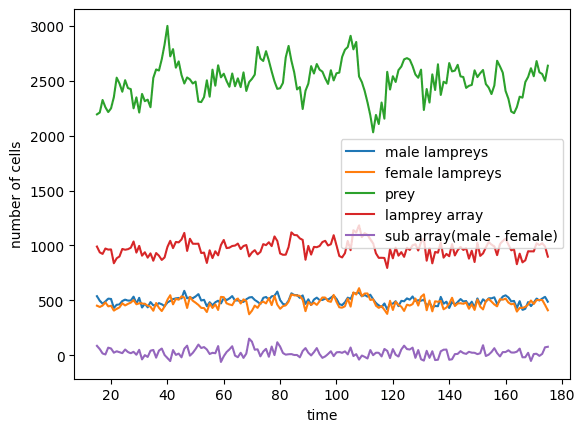
\includegraphics[width=\textwidth]{figures/6_1_figur1.png}
    \caption{$N-\tau_{CA}$ Curve, Under $Env_{A}$}
    \label{fig:sub1}
  \end{subfigure}
  \hfill
  \begin{subfigure}[b]{0.45\textwidth}
    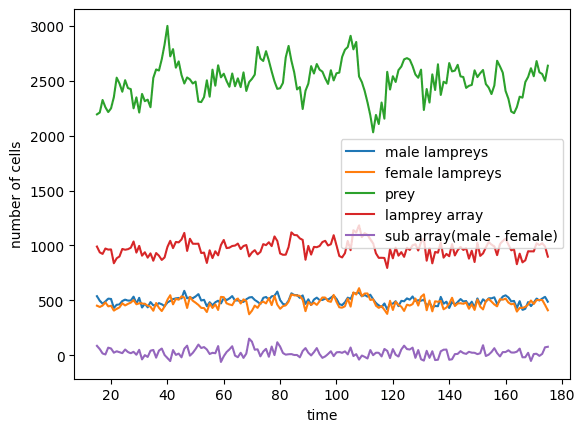
\includegraphics[width=\textwidth]{figures/6_1_figur1.png}
    \caption{$N-\tau_{CA}$ Curve, Under $Env_{B}$}
    \label{fig:sub2}
  \end{subfigure}
  
  \caption{Result of Simulation}
  \label{fig:Result of Simulation}
\end{figure}

From the figures we can see that when the sex ratio is influenced by resource availability, lamprey populations are higher than in cases where the male-female birth rate is 1:1. Prey populations are lower in such scenarios. This gender-regulatory feature makes lampreys more likely to survive and eat more prey. And in resource-rich conditions, the difference between males and females is smaller, sometimes even negative, while in resource-poor conditions it becomes larger. This suggests that in resource-rich environments, lampreys tend to switch to females in order to increase their reproductive rate, whereas in resource-scarce conditions, they tend to switch to males in order to conserve energy and increase their hunting ability in response to reduced food availability. This behaviour closely mirrors real-world ecological dynamics.


\subsection{Apply Model 1: Solve Problem 2}

On the basis of 6.1, we introduced two distinct catastrophes, $D_{prey}$ (a reduction of the prey population to one-third) and $D_{lamp}$ (a reduction of the lamprey population to one-third), at $\tau_{CA} = 66$, as shown in the \textbf{Figures 7-9} below:

\begin{figure}[H]
  \centering
  % 第一行
  \begin{subfigure}[b]{0.45\textwidth}
    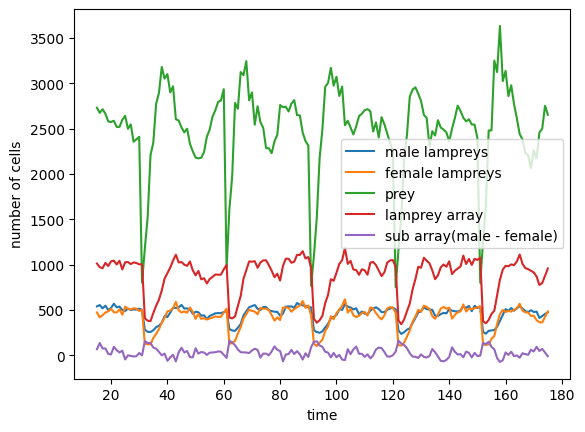
\includegraphics[width=\textwidth]{figures/6_2_figur1.png}
    \caption{$N-\tau_{CA}$ Curve, Under $Env_{A}$, $D_{prey}$}
    \label{fig:sub1}
  \end{subfigure}
  \hfill
  \begin{subfigure}[b]{0.45\textwidth}
    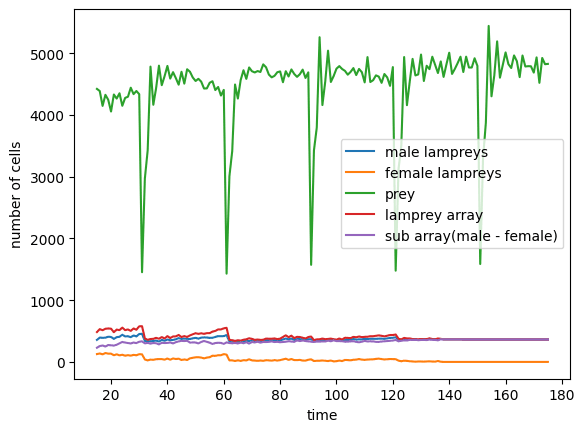
\includegraphics[width=\textwidth]{figures/6_2_figur2.png}
    \caption{$N-\tau_{CA}$ Curve, Under $Env_{B}$, $D_{prey}$}
    \label{fig:sub2}
  \end{subfigure}
  
  \caption{Simulation with Disaster $D_{prey}$}
  \label{fig:Simulation of Disaster}
\end{figure}

\begin{figure}[H]
  \centering
  % 第二行
  \begin{subfigure}[b]{0.45\textwidth}
    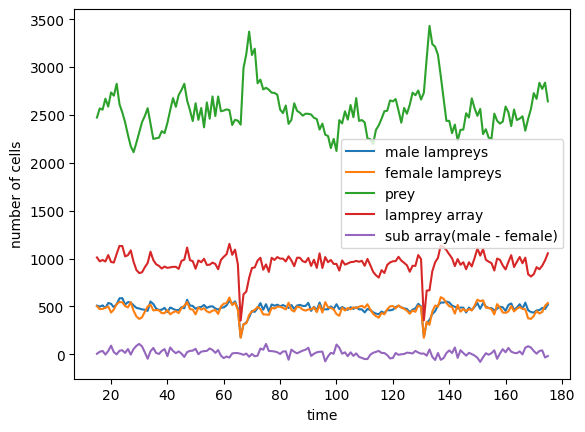
\includegraphics[width=\textwidth]{figures/6_2_figur3.png}
    \caption{$N-\tau_{CA}$ Curve, Under $Env_{A}$, $D_{lamp}$}
    \label{fig:sub1}
  \end{subfigure}
  \hfill
  \begin{subfigure}[b]{0.45\textwidth}
    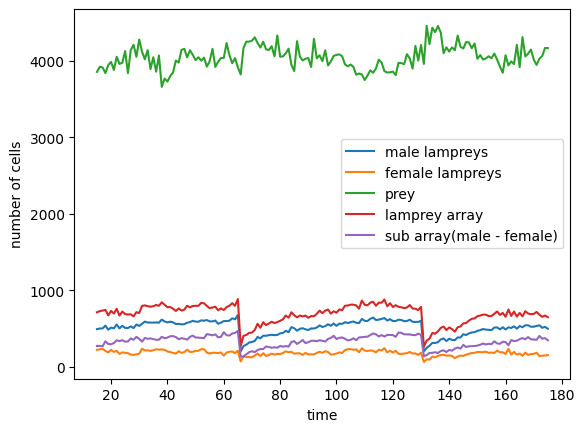
\includegraphics[width=\textwidth]{figures/6_2_figur4.png}
    \caption{$N-\tau_{CA}$ Curve, Under $Env_{B}$, $D_{lamp}$}
    \label{fig:sub2}
  \end{subfigure}

  
  \caption{Simulation with Disaster $D_{lamp}$}
  \label{fig:Simulation of Disaster}
\end{figure}


From the figures, it is evident that in ecosystem $Env_{A}$, regardless of whether it's catastrophe $D_{prey}$ or $D_{lamp}$ , the lamprey population recovers to its original size faster than in ecosystem $Env_{B}$. This suggests that altering the gender ratio helps maintain the stability and resilience of lamprey populations under different environmental conditions.


\begin{figure}[H]
  \centering
  % 第三行
  \begin{subfigure}[b]{0.45\textwidth}
    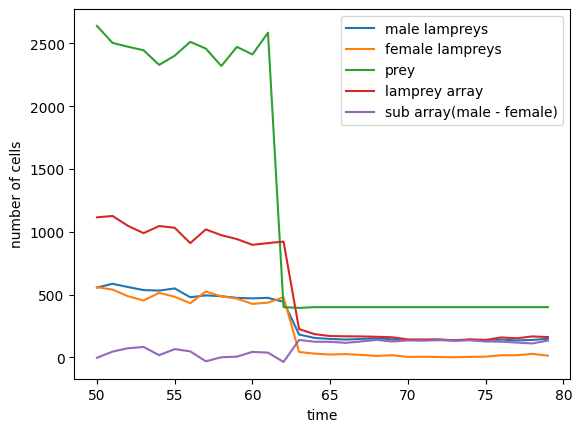
\includegraphics[width=\textwidth]{figures/6_2_figur5.png}
    \caption{$N-\tau_{CA}$ Curve, Under $Env_{A}$, $D_{P}$}
    \label{fig:sub1}
  \end{subfigure}
  \hfill
  \begin{subfigure}[b]{0.45\textwidth}
    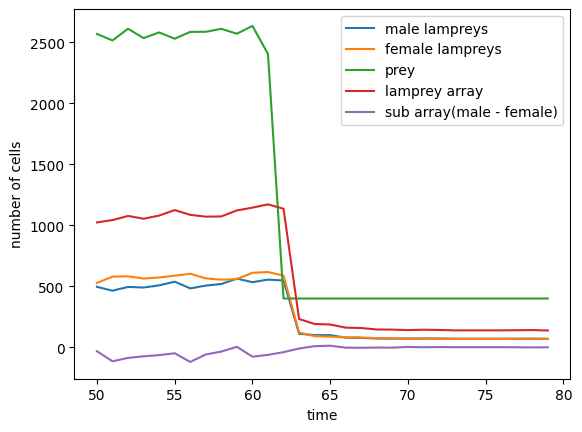
\includegraphics[width=\textwidth]{figures/6_2_figur6.png}
    \caption{$N-\tau_{CA}$ Curve, Under $Env_{B}$, $D_{P}$}
    \label{fig:sub2}
  \end{subfigure}

  \caption{Simulation with Disaster $D_{P}$}
  \label{fig:Simulation of Disaster}
\end{figure}

However, when simulating an extreme catastrophe $D_{P}$ that could potentially lead to extinction, as illustrated below, we see a dramatic decline in the prey population. In such an extreme food scarcity scenario, in ecosystem $Env_{A}$, lampreys primarily transition to males to better survive, leading to a sharp decrease in the female lamprey population and an imbalance in gender ratio. This affects genetic diversity and the long-term population survival capacity. In contrast, in ecosystem $Env_{B}$, even though the lamprey population experiences a sharp decline in extremely scarce food conditions, it still outnumbers the lampreys in ecosystem $Env_{A}$.




\subsection{Apply Model 1 and Model 2: Solving Problem 3}
\subsubsection{Calculating the Weights for Each Indicator}
Based on \textbf{Model 2}, in conjunction with relevant literature and expert recommendations, the pairwise comparison-derived weights are listed in the \textbf{Table 3} following:

\begin{table}[!ht]
    \centering
    \begin{tabular}{ccccc}
    \hline
        \textbf{} & \textbf{\thead{Ecosystem\\ Resilience}} & \textbf{\thead{Ecosystem\\ Resistance}} & \textbf{\thead{Species Population\\ Variability}} & \textbf{\thead{The length of the cycle\\ of change in the population}} \\ \hline
        \textbf{\thead{Ecosystem\\ Resilience}} & 1 & 2 & 3 & 5  \\ 
        \textbf{\thead{Ecosystem\\ Resistance}} & 1/2 & 1 & 1/2 & 2  \\ 
        \textbf{\thead{Species Population\\ Variability}} & 1/3 & 2 & 1 & 2  \\ 
        \textbf{\thead{The length of the cycle\\ of change in the population}} & 1/5 & 1/2 & 1/2 & 1  \\ \hline
    \end{tabular}
    \caption{The Pairwise Comparison-Derived Weights}
    \label{The Pairwise Comparison-Derived Weights}
\end{table}

The constructed pairwise comparison matrix A is as follows:
\begin{align}
A=\left[\begin{matrix}1&2&3&5\\\frac{1}{2}&1&\frac{1}{2}&2\\\frac{1}{3}&2&1&2\\\frac{1}{5}&\frac{1}{2}&\frac{1}{2}&1\\\end{matrix}\right]
\end{align}

We have calculated the consistency index ($CI$) as 0.038 and subsequently computed the consistency ratio ($CR$) as 0.042. Since the $CR$ value is less than 0.1, the consistency of the matrix is considered acceptable. Finally, we have calculated the weight vector $w$:

\begin{align}
w=\begin{bmatrix}
 0.489\\
 0.182\\
0.232\\
0.097
\end{bmatrix}
\end{align}

\subsubsection{Initial Data Processing}
Suppose the system is in a stable state from time $\tau_{CA} = 0$ to $\tau_{CA} = 65$, where the lamprey population and the prey exhibit cyclic variations. At $\tau_{CA} = 66$, a catastrophe occurs, causing the prey to suddenly decrease to one third of its original amount and then return to a stable state after $m$ years. Using \textbf{Model 1}, we simulate three ecosystems: $Env_{A}$, $Env_{B}$ , and $Env_{C}$ . The \textbf{Figure 10} below show changes in prey and lamprey populations over time:


\begin{figure}[H]
  \centering
  % 第一行
  \begin{subfigure}[b]{0.3\textwidth}
    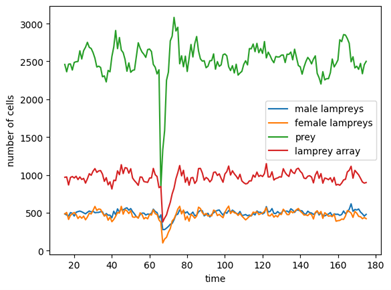
\includegraphics[width=\textwidth]{figures/6_3_figur1.png}
    \caption{$N-\tau_{CA}$ Curve, Under $Env_{A}$}
    \label{fig:sub1}
  \end{subfigure}
  \hfill
  \begin{subfigure}[b]{0.3\textwidth}
    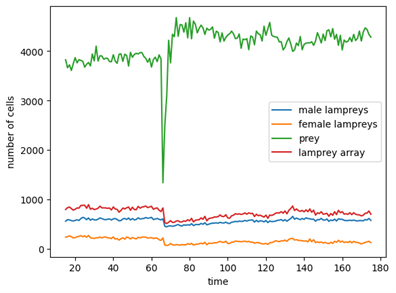
\includegraphics[width=\textwidth]{figures/6_3_figur2.png}
    \caption{$N-\tau_{CA}$ Curve, Under $Env_{B}$}
    \label{fig:sub2}
  \end{subfigure}
  \hfill
  \begin{subfigure}[b]{0.3\textwidth}
    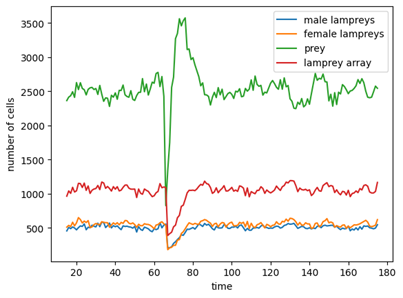
\includegraphics[width=\textwidth]{figures/6_3_figur3.png}
    \caption{$N-\tau_{CA}$ Curve, Under $Env_{C}$}
    \label{fig:sub2}
  \end{subfigure}
  \caption{$N-\tau_{CA}$ Curve, Under different $Env$}
  \label{fig:Simulation of Disaster}
\end{figure}

Assuming a periodicity of $T$ (units: years), the average amplitude of the lamprey population function over time is denoted as $U$, and the prey as $N_V$. The average quantity of lamprey is denoted as $\bar{ N_X}$ , and the average quantity of prey as $\bar{ N_Y}$. After the disaster occurs and the system returns to stability, the lamprey population is denoted as $N_Z$, the prey is denoted as $N_W$, and the time it takes for the system to return to stability after the disaster is denoted as $m$.

Based on the fitting of \textbf{Figure 10}, the original data is as \textbf{Table 4} below:

\begin{table}[!ht]
    \centering
    \begin{tabular}{ccccccccc}
    \hline
        \textbf{Ecosystem} & \textbf{$T$} & \textbf{ $\bar{ N_X}$} & \textbf{$\bar{ N_Y}$} & \textbf{$U$} & \textbf{$N_V$} & \textbf{$m$} & \textbf{$N_Z$} & \textbf{$N_W$} \\ \hline
        \textbf{$Env_{A}$} & 14.50 & 2525.95 & 966.12 & 54.38 & 118.03 & 10 & 2542.82 & 968.84  \\ 
        \textbf{$Env_{B}$} & 9.83 & 3822.12 & 806.90 & 20.21 & 50.21 & 30 & 4264.13 & 702.06  \\ 
        \textbf{$Env_{C}$} & 29.50 & 2498.85 & 1072.02 & 56.22 & 107.96 & 25 & 2780.15 & 1064.37  \\ \hline
    \end{tabular}
    \caption{The Original Data}
    \label{The Original Data}
\end{table}

Calculate the species population variability (a), the length of the cycle of change in the population (b), ecosystem resilience (c), ecosystem resistance (d), resulting in the \textbf{Table 5}:

\begin{table}[!ht]
    \centering
    \begin{tabular}{ccccc}
    \hline
        \textbf{Ecosystem} & \textbf{a} & \textbf{b} & \textbf{c} & \textbf{d } \\ \hline
        \textbf{$Env_{A}$} & 0.1437 & 14.50 & 10 & 0.009494  \\ 
        \textbf{$Env_{B}$} & 0.0675 & 9.83 & 30 & 0.245575  \\ 
        \textbf{$Env_{C}$} & 0.1232 & 29.50 & 25 & 0.105435  \\ \hline
    \end{tabular}
    \caption{Ecosystem-Factors}
    \label{Ecosystem-Factors}
\end{table}

Express the above table in matrix form, denoted as matrix $M_1$:
\begin{align}
M_1=\left[\begin{matrix}0.1437&14.50&10&0.009494\\0.0675&9.83&30&0.245575\\0.1232&29.50&25&0.105435\\\end{matrix}\right]
\end{align}

\subsubsection{Calculating the Ecosystem Stability Score}
According to \textbf{Model 2}, transform $M_1$ into the standardized matrix $M$:
\begin{align}
M=\left[\begin{matrix}0&0.041&0.177&0.420\\0.223&0.028&0&0\\0.060&0.083&0.044&0.249\\\end{matrix}\right]
\end{align}

Finally, based on $M$, we can obtain the stability scores for ecosystems $Env_{A}$, $Env_{B}$, and $Env_{C}$, as \textbf{Table 6}:

\begin{table}[!ht]
    \centering
    \begin{tabular}{cc}
    \hline
        \textbf{Ecosystem} & \textbf{Scores } \\ \hline
        \textbf{$Env_{A}$} & 44.98  \\ 
        \textbf{$Env_{B}$} & 21.89  \\ 
        \textbf{$Env_{C}$} & 33.13  \\ \hline
    \end{tabular}
    \caption{The Stability Scores}
    \label{The Stability Scores}
\end{table}

Based on the final scores, it is evident that lampreys capable of adjusting gender ratios achieve the highest stability scores in the ecosystem, whereas lampreys with an equal male-female birth ratio receive the lowest stability scores, which are less than half of the former's scores. Therefore, lampreys capable of adjusting gender ratios have a significant impact on ecosystem stability, substantially promoting its stability.

\subsection{Improve Model 1: Solve Problem 4}

In \textbf{Model 1} we introduced parasites as predators, but the parasites themselves cannot prey on lampreys, so the lamprey population does not change with variations in parasite numbers. We define the nutrient supply factor $k$ to represent the energy gained by feeding on lampreys. Because different sexes carry different energy reserves, we assign different $k$'s to male and female lampreys. We set up the parasite-as-predator, and the \textbf{Algorithem 1} as follows: 


\begin{algorithm}
\caption{Rules of Parasite as Predator}
\begin{algorithmic}[1]
\State $as\_food\_lampary = N_{male} \times k_m + N_{female} \times k_f$
\State $k_m, k_f = 0.5, 1.5$ \Comment{Male coefficient and Female coefficient}
\State $C_1 = 1.6 + 0.4 \times \text{rand}(), \,\,\,\,\, C_2 = 2.0 + 0.4 \times \text{rand}()$ \Comment{Lower Bound}
\State $l_1, r_1 = l_2, r_2 = 1, 9$ \Comment{Breeding Range and Survive Range}
\If{$\text{state} == 0$} \Comment{Dead state}
    \If{$N_{parasite} == 0$}
        \State \Return 0
    \EndIf
    \If{$(as\_food\_lamprey / N_{parasite} > C_1)$ \textbf{and} $\text{inRange}(l_1, r_1, N_{parasite})$}
        \State \Return 1
    \Else
        \State \Return 0
    \EndIf
\ElsIf{$\text{state} == 1$} \Comment{Alive state}
    \If{$(as\_food\_lamprey / N_{parasite} > C_2)$ 
        \textbf{and} $\text{inRange}(l_2, r_2, N_{parasite})$}
        \State \Return 1
    \Else
        \State \Return 0
    \EndIf
\EndIf
\end{algorithmic}
\end{algorithm}

\begin{figure}[H]
  \centering
  % 第一行
  \begin{subfigure}[b]{0.45\textwidth}
    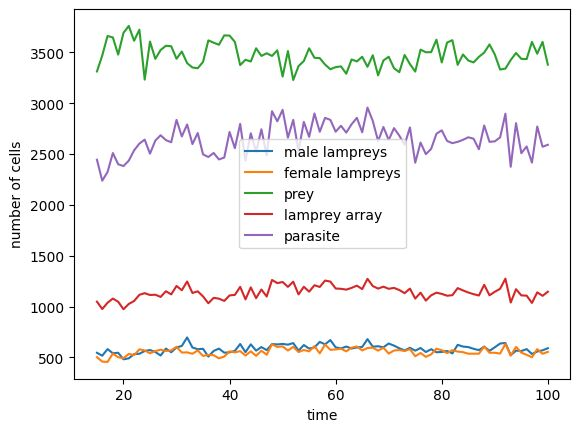
\includegraphics[width=\textwidth]{figures/6_4_figur1.png}
    \caption{$N-\tau_{CA}$ Curve, Under $Env_{A}$}
    \label{fig:sub1}
  \end{subfigure}
  \hfill
  \begin{subfigure}[b]{0.45\textwidth}
    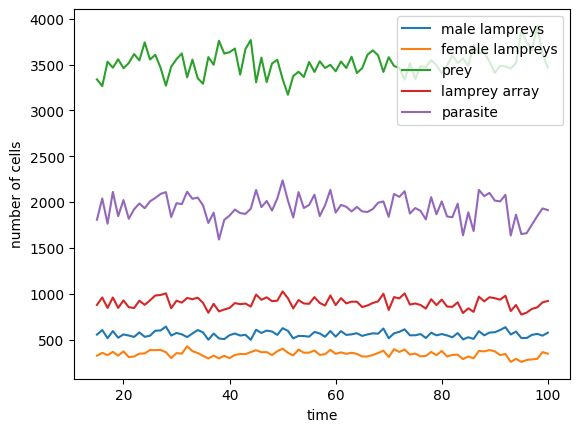
\includegraphics[width=\textwidth]{figures/6_4_figur2.png}
    \caption{$N-\tau_{CA}$ Curve, Under $Env_{B}$}
    \label{fig:sub2}
  \end{subfigure}

  \caption{Curve Containing the Number of Parasites}
  \label{fig:Simulation of Disaster}
\end{figure}
 
We simulated different parasite populations in ecosystem $Env_{A}$ and ecosystem $Env_{B}$ by using this improved model1, which is displayed in \textbf{Figure 11}. 

We found that in ecosystem $Env_{A}$, the parasite survival exceeds that in ecosystem $Env_{B}$, leading to the following conclusion: gender ratio variability results in an increased population of parasites.  

\section{Sensitivity Analysis and Stability Analysis}
\subsection{Sensitivity Analysis}
In 4.3, we performed a qualitative analysis to obtain reasonable estimates for most of the parameters. However, they are still difficult to estimate computationally and in this section we will perform a sensitivity analysis by adjusting these parameters. 

First, we analyse the sensitivity of $pre_m$ (the predatory ability of male lampreys) and $res_m$ (the resource requirements of male lampreys). As \textbf{Figure 12}.

\begin{figure}[H]
  \centering
  % 第一行
  \begin{subfigure}[b]{0.45\textwidth}
    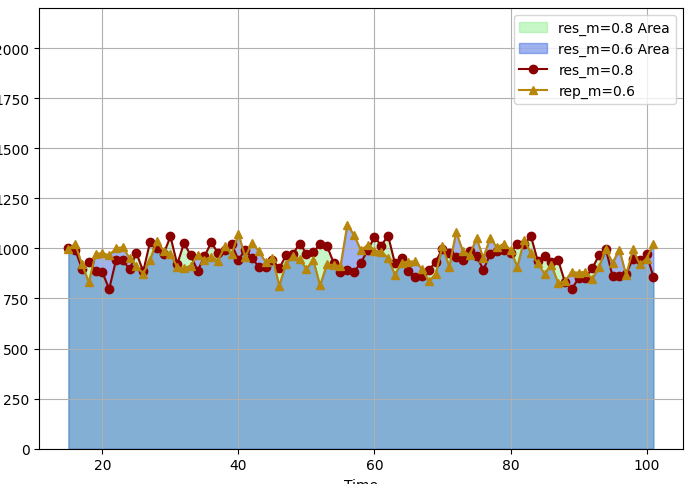
\includegraphics[width=\textwidth]{figures/7_1_figur1.png}
    \caption{Effect of Value of $Res_{req}$}
    \label{fig:sub1}
  \end{subfigure}
  \hfill
  \begin{subfigure}[b]{0.47\textwidth}
    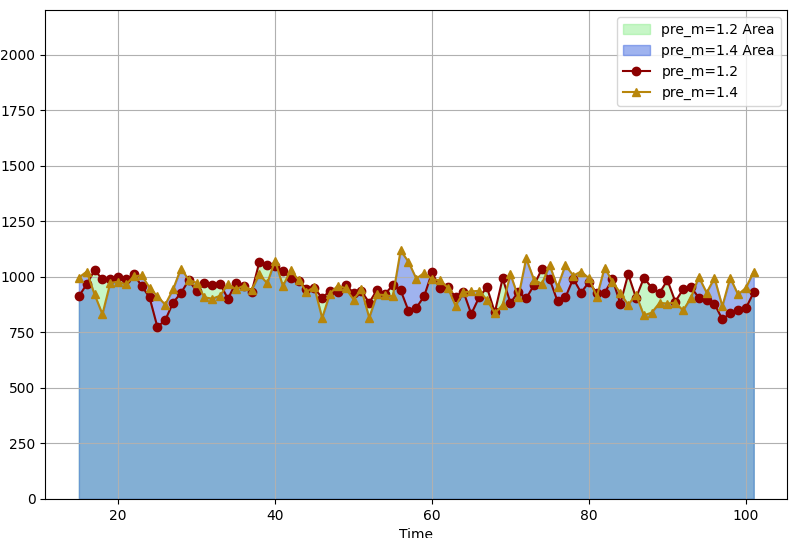
\includegraphics[width=\textwidth]{figures/7_1_figur2.png}
    \caption{Effect of Value of $Prey_{ab}$}
    \label{fig:sub2}
  \end{subfigure}

  \caption{ Effect of Value of $Res_{req}$ and $Prey_{ab}$}
  \label{fig:Simulation of Disaster}
\end{figure}

Then, we analyze the sensitivity of $rep_m$ (which is the reproductive capacity of male lampreys).  As \textbf{Figure 13}.


\begin{figure}[H]
  \centering
  % 第一行
  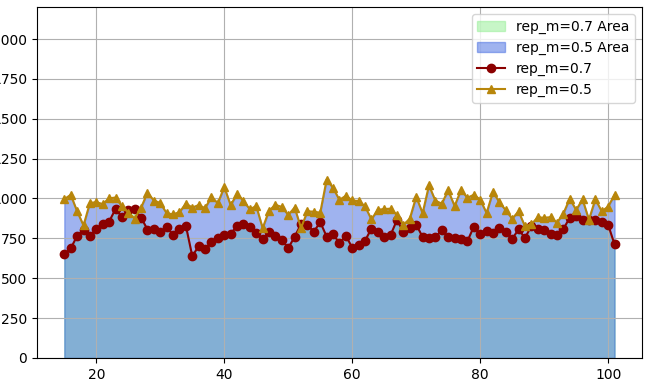
\includegraphics[width=0.5\textwidth]{figures/7_1_figur3.png}
  \caption{Effect of Value of $Rep_{capa}$}
  \label{fig:Simulation of Disaster}
\end{figure}

Our models perform well in sensitivity analysis for most parameters. This shows that our model has good long-term stability. However, the sensitivity of the fertility parameter is high, which we need to improve.


\subsection{Stability Analysis}
We choose an initial value for the model (Initial values for prey simulation). We perturb this value by 5\%. This means that the initial value of 2400 for the prey simulation was perturbed to $2400\times (1\pm 5\%)$ and three sets of lamprey population simulation data were observed. We then use these data to test the stability of our model and the decision model. The results are shown in \textbf{Figure 14}:

\begin{figure}[H]
  \centering
  % 第一行
  \begin{subfigure}[b]{0.47\textwidth}
    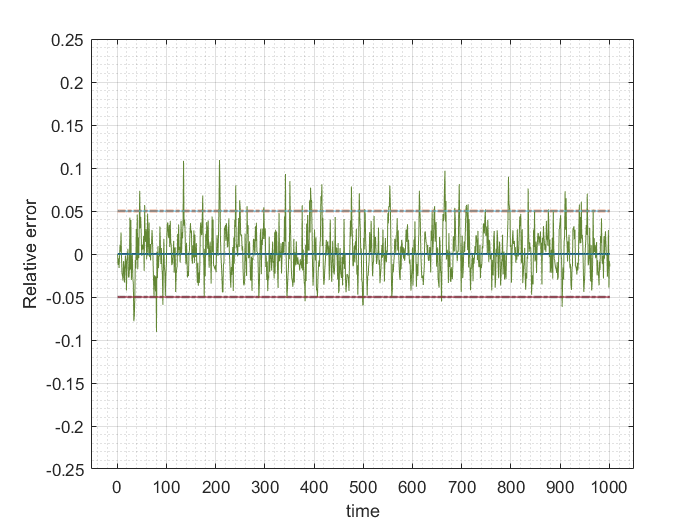
\includegraphics[width=\textwidth]{figures/7_2_figur1.png}
    \caption{Relative Error}
    \label{fig:sub1}
  \end{subfigure}
  \hfill
  \begin{subfigure}[b]{0.49\textwidth}
    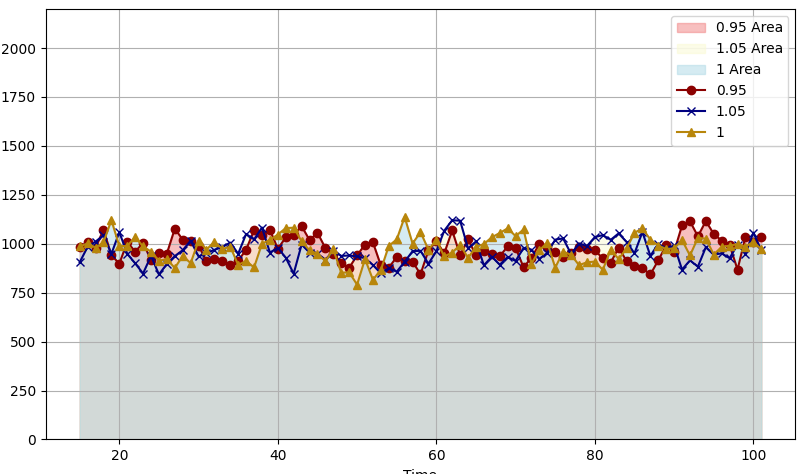
\includegraphics[width=\textwidth]{figures/7_2_figur2.png}
    \caption{Absolute error}
    \label{fig:sub2}
  \end{subfigure}

  \caption{Error Analysis Visualisation}
  \label{fig:Simulation of Disaster}
\end{figure}

We show the effect of fitting more volatile and representative data. The results indicate that the relative errors are mostly limited to 5\%, suggesting that the model remains stable even when the initial quantities are altered.



\section{Model Evaluation and Further Discussion}
\subsection{Strengths}
\begin{itemize}
    \item In the simulation model with environmental sex determination, we used the Cellular Automata (CA) model, which offered a simple yet powerful approach to modeling complex systems, allowing for the exploration of emergent phenomena from basic rules. 
    \item  CA can demonstrate self-organizing behavior, making them useful for studying pattern formation and evolution in natural and artificial systems. 
    \item In the ecosystem stability assessment model, we used AHP-TOPSIS, which combined AHP's ability to break down complex decision problems into a hierarchical structure with TOPSIS's efficient ranking mechanism to provide a thorough evaluation approach.
    \item AHP allows for subjective judgments in assigning weights to criteria, while TOPSIS objectively evaluates the alternatives based on those criteria, making the combined method flexible in accommodating different decision-making scenarios.
    \item We do not need to stick strictly to the data collected; instead, we can use the results simulated by this model to better analyse and compare the effects of lampreys with different sex ratios on the ecosystem, the advantages and disadvantages of lampreys, etc.
\end{itemize}

\subsection{Weaknesses}
\begin{itemize}
    \item CA models might oversimplify complex systems, potentially overlooking critical dynamics and leading to inaccurate representations. For example, we only considered the main factors, such as reproductive capacity and resource requirements, but did not take into account other minor factors, such as the natural mortality of lampreys due to changes over time and the effects of inorganic ecosystems.
    \item AHP's reliance on subjective judgments for assigning weights can introduce bias into the decision-making process, affecting the overall objectivity. The outcomes of the AHP-TOPSIS method can be highly sensitive to slight changes in the weights as-signed to criteria, requiring careful consideration and justification of the weights used.
    \item High sensitivity of certain parameters, such as Reproductive Capacity, indicates that minor changes in this parameter can significantly affect the model's output. It can lead to increased uncertainty in predictions, making model calibration to empirical data challenging.
\end{itemize}

\subsection{Further Discussion}
Finally, we also tried to extend the 2-D model to a 3-D environment. \textbf{Figure 15} below is our simulation result. The empty area represents the absence of organisms, while the blue sphere represents a surviving male lamprey and the green sphere represents female's.

%%%%%%%% 图片 %%%%%%%%
\begin{figure}[H]  % 图片
\small
\centering  % 居中
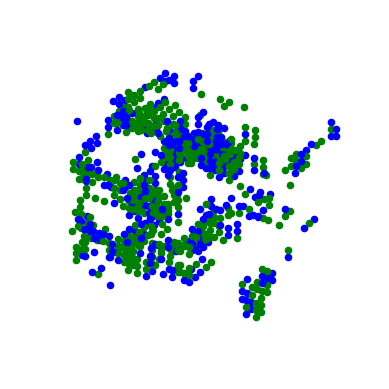
\includegraphics[width=7cm]{figures/3dsimulation.png}  % 引入图片源
\caption{3d-Simulation} \label{fig:Lamprey}  % 标题与标签
\end{figure}  % 图片结束
%%%%%%%% 图片 %%%%%%%%

\section{Conclusion}

By establishing the simulation model with environmental sex determination and the ecosystem stability assessment model, we have perfectly met the requirements of question, drawing a series of conclusions about the impact of lampreys changing its gender:
\begin{itemize}
    \item When the population of lampreys can alter its sex ratio, there will be less prey and more lampreys.

    \item Advantages: Altering the gender ratio helps maintain the stability and resilience of lamprey populations under different environmental conditions.

    \item Disadvantages: When lampreys are in an extreme food scarcity scenario, there will be  a sharp decrease in the female lamprey population and an imbalance in gender ratio, which affects genetic diversity and the long-term population survival capacity.

    \item Lampreys capable of adjusting gender ratios have a significant impact on ecosystem stability, substantially promoting its stability.

    \item Changes in the sex ratio of lampreys can lead to increased parasite populations.
\end{itemize}






\begin{thebibliography}{99}
\bibitem{1} Johnson, Nicholas S., William D. Swink, and Travis O. Brenden. "Field study suggests that sex determination in sea lamprey is directly influenced by larval growth rate." Proceedings of the Royal Society B: Biological Sciences 284, no. 1851 (2017): 20170262.
\bibitem{2} Purvis, Harold A. Variations in growth, age at transformation, and sex ratio of sea lampreys reestablished in chemically treated tributaries of the Upper Great Lakes. No. 35. Ann Arbor, MI: Great Lakes Fishery Commission, 1979.
\bibitem{3} Toffoli, Tommaso, and Norman Margolus. Cellular Automata Machines: A New Environment for Modeling. Cambridge, MA: MIT Press, 1987.
\bibitem{4} Schiff, Joel L. Cellular Automata: A Discrete View of the World. Hoboken, NJ: Wiley \& Sons, Inc, 2011.
\bibitem{5} "Mathematical Modeling of Biological Pattern Formation." In Cellular Automaton Modeling of Biological Pattern Formation, 45-56. Boston, MA: Birkhäuser Boston, 2005.
\bibitem{6} https://fishbase.se/summary/SpeciesSummary.php?ID=2530\&AT=sea+lamprey
\bibitem{7}  Applegate, Vernon C., and M. L. H. Thomas. "Sex ratios and sexual dimorphism among recently transformed sea lampreys, Petromyzon marinus Linnaeus." Journal of the Fisheries Board of Canada 22, no. 3 (1965): 695-711.
\bibitem{8} Dhamelincourt, M., et al. "Sea Lamprey (Petromyzon marinus L.) Nests Do Not Affect Stream Functionality Despite Increasing Physical Heterogeneity." Aquatic Sciences, vol. 85, 2023, p. 49. 
\end{thebibliography}



\newpage
\begin{appendices}
Here is the main function of simulation programme we used in our model as follow.\\
\textbf{\textcolor[rgb]{0.98,0.00,0.00}{Input python source:}}
\begin{lstlisting}[language=python]
# main function
if __name__ == "__main__":
    state = cellState(nx, ny)
    state.random_lampreys(male_init_number, female_init_number)
    state.random_prey(prey_init_number)
    state.random_predator(predator_init_number)
    state.plot_state(picture_style, -1)

    male_array.append(state.lampreys_male_alive)
    female_array.append(state.lampreys_female_alive)
    prey_array.append(state.prey_alive)
    predator_array.append(state.predator_alive)


    for i in range(0, nt):
        state.updateState()

   
        # append the number of cells to the array
        male_array.append(state.lampreys_male_alive)
        female_array.append(state.lampreys_female_alive)
        prey_array.append(state.prey_alive)
        predator_array.append(state.predator_alive)

        # plot the state of the cells
        if i % 20 == 19:
            state.plot_state(picture_style, i)

        # check if the number of cells is conserved
        if (
            state.lampreys_female_alive
            + state.lampreys_male_alive
            + state.prey_alive
            + state.predator_alive
            > 3 * nx * ny
        ):
            print("Error: the number of cells is not conserved")
            break

    print("The end of the simulation")
\end{lstlisting}

Here is the method of update() in simulation programme we used in our model as follow.\\
\textbf{\textcolor[rgb]{0.98,0.00,0.00}{Input python source:}}
\begin{lstlisting}[language=python]
# update the state of the cells
def updateState(self):
    new_lampreys = np.zeros((self.nx, self.ny))
    new_prey = np.zeros((self.nx, self.ny))
    new_predator = np.zeros((self.nx, self.ny))
    new_male_alive = 0
    new_female_alive = 0
    new_prey_alive = 0
    new_predator_alive = 0

    # for the lampreys
    for i in range(self.nx):
        for j in range(self.ny):
            new_lampreys[i][j] = nextCellLampary(
                self.countCellState(i, j), self.lampreys[i][j], "lampary"
            )
            if new_lampreys[i][j] == 1:
                new_male_alive += 1
            elif new_lampreys[i][j] == 2:
                new_female_alive += 1

    self.lampreys = new_lampreys.copy()
    self.lampreys_male_alive = new_male_alive
    self.lampreys_female_alive = new_female_alive

    # for the prey and the predator
    for i in range(self.nx):
        for j in range(self.ny):
            # for the prey
            new_prey[i][j] = nextCellLampary(
                self.countCellState(i, j), self.prey[i][j], "prey"
            )
            if new_prey[i][j] == 1:
                new_prey_alive += 1
            new_predator[i][j] = nextCellLampary(
                self.countCellState(i, j), self.predator[i][j], "predator"
            )
            if new_predator[i][j] == 1:
                new_predator_alive += 1

    self.prey = new_prey.copy()
    self.prey_alive = new_prey_alive
    self.predator = new_predator.copy()
    self.predator_alive = new_predator_alive
\end{lstlisting}

\end{appendices}

\end{document}
%% 
%% This work consists of these files mcmthesis.dtx,
%%                                   figures/ and
%%                                   code/,
%% and the derived files             mcmthesis.cls,
%%                                   mcmthesis-demo.tex,
%%                                   README,
%%                                   LICENSE,
%%                                   mcmthesis.pdf and
%%                                   mcmthesis-demo.pdf.
%%
%% End of file `mcmthesis-demo.tex'.
